\documentclass[11pt,a4paper]{ltjsreport}
\usepackage{luatexja-fontspec}
\usepackage{tocloft}
\usepackage{fancyhdr} % ヘッダ・フッター用
\usepackage{makeidx} %目次表目次図目次の出力
\usepackage{lscape}
\usepackage{url} %参考文献のURL途中改行
\usepackage{tikz} %TeXで図を描きたい人用
\usepackage{amsmath} %数式用
\usepackage{titlesec} %chapterなどのタイトルフォントの大きさを調整したい時用
\usepackage{pdfpages} % PDF挿入用のパッケージ

% \titleformat{\chapter}[display]{\huge\bfseries}{第\ \thechapter \ 章}{40pt}{}[]
%jsreportだとChapterのフォントサイズがデカくて恥ずかしいのでここで調整している

\newcommand{\bhline}{\noalign{\hrule height 1.2pt}} % 太い横線の定義(表の上部の太線用)
\renewcommand{\baselinestretch}{1.0}

%------章はじめのページにヘッダーとフッターを付けるための処理
\makeatletter
\renewcommand{\chapter}{%
    \if@openleft\cleardoublepage\else
    \if@openright\cleardoublepage\else\clearpage\fi\fi
    %\plainifnotempty %元: \thispagestyle{plain}
    \global\@topnum\z@
    \if@english \@afterindentfalse \else \@afterindenttrue \fi
    \secdef
    {\@omit@numberfalse\@chapter}%
    {\@omit@numbertrue\@schapter}}
\makeatother
%------ここまで章はじめのページにヘッダーとフッターを付けるための処理

% 目次のインデント調整
\cftsetindents{chapter}{0em}{5em} % 章
\cftsetindents{section}{2em}{3em} % 節
\cftsetindents{subsection}{4em}{3em} % 小節

\begin{document}

%------表紙
\begin{titlepage}
    \null
    \vfil
    \begin{center}
        {\huge\textbf{チャットの吹き出しにおけるアニメーション\\効果とインタラクションの研究}\par}\vskip 8em minus 2em %2行にする場合は、象の卵の\\デザイン みたいに\\をいれる
        % \begin{table}[htb]
        %     \renewcommand{\arraystretch}{1.3}
        %     \centering
        %     \begin{tabular}
        %         {@{\vrule width 1.8pt\ }c|c|c@{\ \vrule width 1.8pt}}
        %         \noalign{\hrule height 1.8pt}
        %         \multicolumn{3}{@{\vrule width 1.8pt}c@{\ \vrule width 1.8pt}}{\large \   筑波大学 デザイン学学位プログラム  \ } \\
        %         \multicolumn{3}{@{\vrule width 1.8pt}c@{\ \vrule width 1.8pt}}{\textbf{{\Large{}}}}              \\ \hline
        %         \multicolumn{2}{@{\vrule width 1.8pt}c|}{\large \ 卒 業 年 度} & \large 令和6年度                        \\ \hline
        %         \multicolumn{2}{@{\vrule width 1.8pt}c|}{\large \ 指 導 教 員} & \large 山田博之                         \\
        %         \noalign{\hrule height 1.8pt}
        %     \end{tabular}
        % \end{table}

        \par \vskip 10em
            {\Large{筑波大学 人間総合科学術院 人間総合科学研究群\\デザイン学学位プログラム 博士前期課程}}
        \vskip 2em
            {\Large{徳永 萌}\par}\vskip 2em minus 2em
        \vskip 2em
            {\Large{令和 年 月 日}}\vskip 2em minus 2em
    \end{center}
    \vfil
    \setcounter{page}{1}
\end{titlepage}
\newpage
%------ここまで表紙

%------要旨
\thispagestyle{empty}

\noindent
\textbf{あらまし\ }
オンライン上でコミュニケーションをとる手段は様々であり、その代表的なツールとして
メッセージアプリによるテキストチャットやイラストなどを使用したスタンプ機能、リアクション機能などが挙げられる。
本研究ではこのような既存の機能に対しユーザー同士が相互にインタラクションすることができる機能を
搭載したツールの提案・効果の調査を行った。

非言語情報をメッセージアプリ上で伝える手段は多くはなく、

\vskip 2em minus 2em
\noindent
keyword, keyword, keyword, keyword, keyword, keyword
%------ここまで要旨

%------目次
\clearpage
\setcounter{page}{0}\pagenumbering{roman}\pagestyle{plain} %ローマ数字のページ番号セット
\setcounter{tocdepth}{2} % \subsection まで目次に表示
\tableofcontents%目次
\listoffigures%図目次
\listoftables%表目次
\clearpage
%------ここまで目次

\setcounter{page}{0}\pagenumbering{arabic} %アラビア数字のページ番号セット

%------本文のヘッダとフッタの設定
\pagestyle{fancy}
\fancyhead{} % clear all header fields
% \lhead{} %ヘッダ左
\renewcommand{\chaptermark}[1]{\lhead{第\ \thechapter\ 章~~~#1}{}}
\chead{} %ヘッダ中央
\rhead{\thepage} %ヘッダ右 ページ番号
\lfoot{} %フッタ左
\cfoot{} %フッタ中央.ページ番号を表示
% \rfoot{造形・メディアデザインコース} %フッタ右
\renewcommand{\footrulewidth}{0.5pt} %フッタの罫線
%------ここまで本文のヘッダとフッタの設定

%------本文開始
\chapter{はじめに}
\section{研究の背景}
本節では本研究の背景としてSNSの利用率、
テキストベースのコミュニケーションにおける非言語情報の伝達
の2点について述べる。

\subsection{SNSの利用率}
今やオンライン上でコミュニケーションを行うことは現代の生活に欠かせないものである。
携帯電話が登場してからコミュニケーションの手段は格段に増え、近年ではスマートフォンの利用者は
全世帯の97.5%とされている\cite{Web1}。\\
総務省の「令和5年度情報通信メディアの利用時間と情報行動に関する調査」によれば
2023年時点における10代、20代のソーシャルメディアの平均利用時間は平日で70分を超え、休日では80分を超えるという結果となっている。
20代の休日のソーシャルメディアの平均利用時間は100分を超えており、20代のメールの利用率が平日・休日ともに平均30分前後なのに対し
非常に高い利用率となっている\cite{Web1}。平日、休日を合わせた平均利用時間を図\ref{figure:graph2}に示す。

\begin{figure}[htbp]
    \begin{center}
        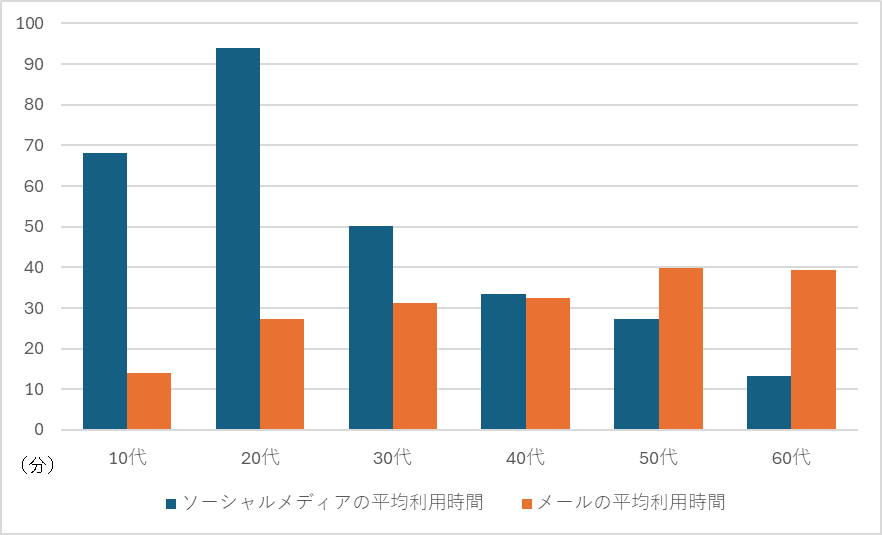
\includegraphics[width=120mm]{PDF/graph_2.pdf}
        \caption{ソーシャルメディア・メールの平均利用時間}
        \label{figure:graph2}
    \end{center}
\end{figure}

これらのデータから、スマートフォンの普及により人々のコミュニケーションの手段は変遷しており、電子メールや電話といった手段から、
メッセージアプリやSNSといったコミュニケーションツールが主な手段に変わったことが分かる。

\subsection{コンピュータを介したコミュニケーションにおける非言語情報の伝達}
人と人との関わりにおいて、感情がどれだけ効果的に伝達され、どれだけ正確に理解されるかは、対人関係のみならず、
個人の幸福にも大きな影響を与える\cite{book_Susan}。対面コミュニケーションでは、表情、身振り、
声のトーンといった豊富な感情的手がかりを活用し、会話の感情的ニュアンスを伝え、理解することが可能である。

一方、コンピュータを介したコミュニケーション(Computer-Mediated Communication, CMC)環境では、
対面における非言語情報の多くが制限される。
しかしその利便性から、前述のようにテキストを用いたコミュニケーションは日常生活で頻繁に行われており、
メッセージアプリの利用は欠かせないものとなっている。
X(旧Twitter)やLINEをはじめとするSocial Networking Service(SNS)の利用者数は増加の一途をたどっており、
特にメッセージ機能を有するアプリケーションの利用率が高い\cite{Web1}。

非言語情報の制限はテキストベースのインスタントメッセージ(Instant Messaging, IM)
アプリケーションにおいて顕著であり、対話者は豊かな感情表現を行うことが難しい\cite{Thesis_Joseph}。
その結果、受け手が会話相手を評価する手がかりも限られるため、
相手の性格や意図について理想化されたイメージが形成されやすい傾向がある\cite{Thesis_Joseph2}。
さらに、テキストベースのCMCでは感情的な喚起が弱く、
メッセージの感情的トーンが誤解される可能性が高くなることが指摘されている \cite{Thesis_Joseph}。
このような環境では、相互理解や感情の伝達、合意形成が非言語的手がかりなしには困難となり、
誤解や対人関係のトラブルを招く可能性がある\cite{Thesis_Morimoto}。

また、SNS上のトラブルは「SNS疲れ」を引き起こし、長時間の利用に伴う精神的・身体的疲労や、
知人の発言に返答する義務感が生じる現象が報告されている\cite{Thesis_Okamoto}。これらの課題を解決するため、
スタンプやリアクション、ボイスメッセージといった非言語的手がかりを補完する手段が導入されている。
これらは、表情や動作といった対面コミュニケーションで得られる非言語情報を文字や記号、イラスト、
音声などで表現することで、コミュニケーションの円滑化を図っている。

しかし、既存のメッセージ機能で利用可能な非言語情報の表現手段は、感情を表現するイラストや絵文字、
ジェスチャーなどに限られており、その効果的な活用にはさらなる検討が必要である。
本研究では、既存のメッセージアプリにおける機能を拡張し、非言語情報の伝達をより効果的に行うための手法を提案し、
その有効性を評価することを目的とする。

\section{研究の目的}
本研究の目的は、メッセージアプリ上の吹き出しにインタラクティブな機能を搭載し、
対面の会話で生じる非言語情報をメッセージアプリ上で表現できるかを評価することである。
従来のテキストベースのやり取りでは伝わりにくい感情や動作を、吹き出しに触れ合うことでより自然に表現し、
コミュニケーションの質を向上させる。吹き出しを通じた触れ合いは、
お互いが同じものに触れているような感覚を生み出し、親密度を高め、相手との仲を深めることが期待される。
従来のスタンプや絵文字では伝えきれない微細な感情や、会話の中での小さな動作
(例えば、軽い突っ込みのような表現)が吹き出しを通じて効果的に伝わると考えられる。
これにより、相手からのリアクションに対してより具体的な返答が生まれ、コミュニケーションの深化が期待される。
また、ビデオ通話や通話が難しい状況下、あるいはそれを望まない場面でも、この手法を用いることで相手の存在を感じ、
コミュニケーションのぬくもりを保つことが可能であると考える。
これにより、異なる状況下での柔軟で温かいコミュニケーションが実現される。
本研究では新しいメッセージアプリの機能を通じて、ユーザーにより深いコミュニケーション経験を提供し、
感情表現の幅を拡げることを目指している。

\section{本論文の構成}
本論分は、本章を含め5章で構成されている。第2章では本研究と関連する研究・事例について述べ、
本研究の位置づけを明らかにする。第3章では実験内容および評価方法について述べる。
第4章では結果をもとに分析・考察し、第5章で結果としてまとめている。



\chapter{関連研究・事例}

\section{各メッセージアプリにおける感情表現の事例}
本節では各メッセージアプリにおける感情表現の事例について述べる。

\subsection{フェイスマーク(Smiley)、絵文字}
小澤ら\cite{Thesis_Ozawa}によればEmojiがUnicodeに採用された2010年以前には、文章中における感性情報の伝達には、
文字や記号を組み合わせた電子表情である「フェイスマーク(Smiley)、顔文字」が主に使われていた。
\texttt{:-)}のような「コロン」や「ハイフン」などの組み合わせで構成するSmileyは、
1970年代に欧米で文章だけでは表現しきれない感情のニュアンスを補うものとして誕生した。
これが、キーボード入力が一般的となりつつあった当時の日本の文化にも溶け込み、
フェイスマークと呼ばれて定着した。 Smileyでは: -)のように顔を転倒して表すのに対して、
フェイスマークでは\texttt{(\textasciicircum-\textasciicircum)}のように正立のまま表す場合が多い。
フェイスマークや絵文字はテキストベースのコミュニケーションツールにおいて非言語情報を伝達することが期待される一方で、
送り手の感情が正しく伝達されているという確証が得られていないのが実情である。
すなわち、多義性があり意味が曖昧なため安易に使うと誤解を生む危険性が指摘されている。\\

テキストのみのチャットでユーザーの感情状態を検出し、絵文字を使ってそれを伝える新しい方法も提案されている。
Liuら\cite{Thesis_Liu}は、ユーザーの顔の表情を基にテキストメッセージに絵文字を付与するシステム「ReactionBot」を提案した。
ReactionBotは、ReactionBotはSlack上で動作するチャットボットであり、
ウェブカメラを利用してユーザーの顔の表情を検出し、それに応じた絵文字をメッセージに自動付与する機能を持つ。
設計にはMicrosoftのEmotion APIを活用し、怒り、喜び、悲しみ、驚き、嫌悪などの
7つの基本感情を検出する仕組みを構築している。
結果として、ReactionBotは手動での絵文字入力を減少させ、感情表現を効率的に補助することが示された。
特に、顔の表情に基づく絵文字は、自然かつ正確な感情伝達を可能にし、
ユーザー自身の感情への認識を高める効果も確認された。
しかし、予想に反して、ReactionBotの利用はペア間の行動的相互依存性(社会的存在感)を低下させることが明らかとなった。
これは、システムが感情表現を自動化することで直接的な反応が減少し、
相手とのつながりが希薄に感じられることが要因と考えられる。

\subsection{LNEのスタンプ・リアクション機能}
LINEの月に1回以上利用のあるMAU(Monthly Active User)は9,500万人(2023年6月末時点)を超えており、
これは日本の総人口(1億2450万人)の約75%にあたる。LINEの利用年代は10代〜70歳以上までと幅広く、
日本のコミュニケーションアプリとして圧倒的なトップシェアを誇るサービスである\cite{Web2}。
LINEを主としたメッセージアプリは主に文字によってやり取りが行われるため、
対面や電話での会話と違い頷き等のジェスチャーや表情、声の調子といった非言語情報はLINE上では伝達されない。
これらの非言語情報の欠落を補完するものとしてLINEのスタンプ機能やリアクション機能が挙げられる(図\ref{figure:LINE_stamp})。
スタンプ機能には、対面会話における非言語コミュニケーションの代替効果があり、
非言語情報の欠落を補完する役割を持つと考えられる。\cite{Thesis_Morimoto}
また、リアクション機能は相手に通知されないため、スタンプ機能に比べより気軽に使用できる機能である。
LINEのような同期型のメッセージアプリでは話題の変化が激しく、
会話に対する相槌が対応するメッセージと離れて送信される場合もあるため\cite{Thesis_Morimoto}、
リアクション機能は相槌のような役割も持つと考えられる。
また森本はLINE等のメッセージアプリで採択されている「スタンプ」についても感情表現やニュアンスの表現として使用されていた顔文字や絵文字と比べ、
言葉にするのが難しい生の感情を曖昧な印象として表現・伝達することを可能にし、
テキストのみのコミュニケーションであった無機質なやり取りを人間味のあるコミュニケーションに変化させたと述べている\cite{Thesis_Morimoto}。

\begin{figure}[htbp]
    \begin{center}
        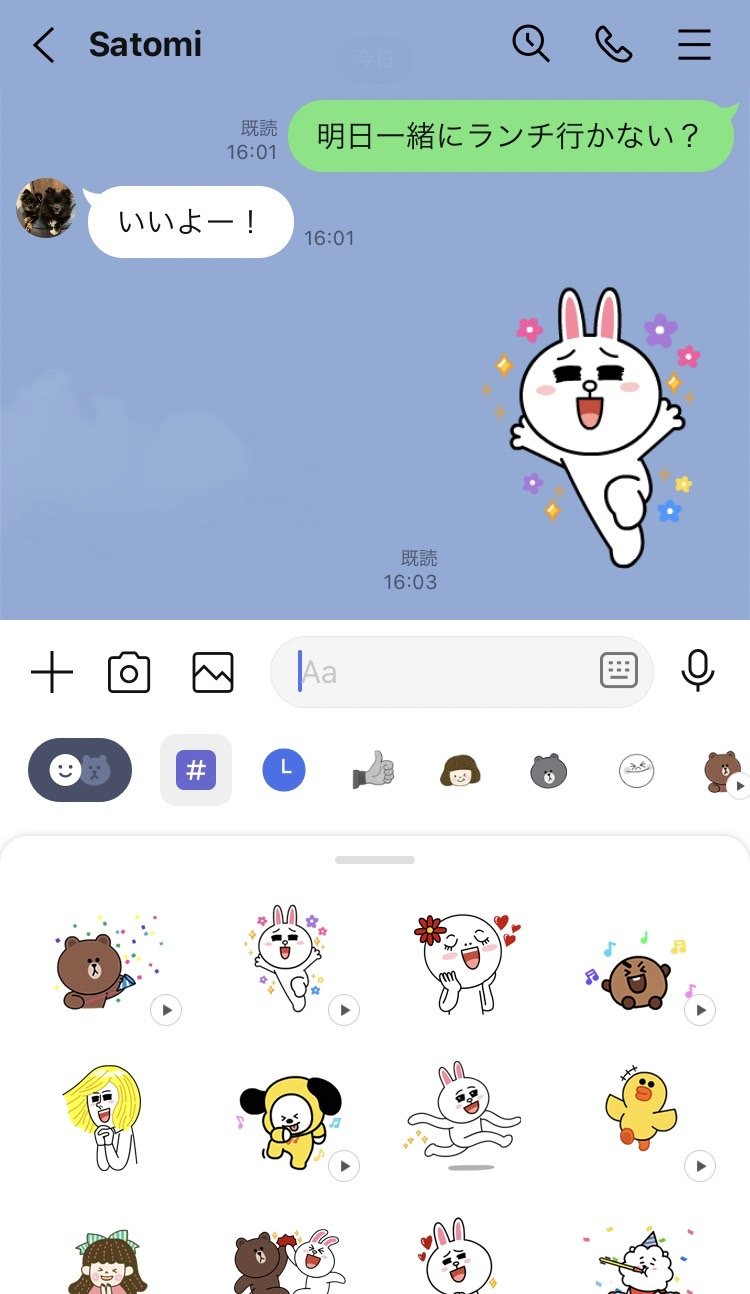
\includegraphics[width=50mm]{PDF/LINE_stamp.jpg}
        \caption{LINEのスタンプ機能}
        \label{figure:LINE_stamp}
    \end{center}
\end{figure}

\subsection{LINE}

\subsection{LINE}

\subsection{LINE}

\section{オンライン上のコミュニケーションにおける感情表現の事例}
本節ではオンライン上のコミュニケーションにおける感情表現の事例について述べる。


\subsection{オンラインゲーム内でのコミュニケーション}
オンラインゲーム内で吹き出しにアイコンを付けたり吹き出しの形状を変化させる機能や(図〇)、
吹き出しの色や形を変化させ感情表現を図る研究が行われている\cite{Thesis2}。
このように吹き出しに変化を付けコミュニケーションを図る事例は存在するが、
吹き出しに触れることでコミュニケーションを図る事例は見られなかったため今回提案・調査する。

\section{メッセージアプリにおける感情伝達の手法に関する研究}
本節ではメッセージアプリにおける感情伝達に関する既存研究について述べる。

\subsection{吹き出しの色や動きについての調査}
野村ら\cite{Thesis_Nomura}はWeb上で円滑なコミュニケーションを行うための既存のメッセージアプリに付随する表現手段を抽出、
整理するとともに、それらの表現手段および表現方法と感情伝達との関係を明らかにした。
この研究ではメッセージアプリでの感情伝達の表現手段として「吹き出し」に着目し、
色や動きを変えることで感情の有効な表現手段を調査した。「吹き出し・文字の動き」、
「吹き出し・文字の動きの周期」、「吹き出しの形状」、「吹き出しの色」の4種類を感情表現の伝達手段として選定した。
感情は「喜び」、「怒り」、「悲しみ」、「驚き」、「恐怖」、「嫌悪」の6種類に対し調査を行った(図\ref{figure:gazou1})。
ポール・エクマンが提唱した「表情から感情の分類を行っているエクマン理論」をもとに選定し、
1種類の感情ごとにスマートフォン8台を用いて8サンプルを提示し各感情が伝わる順番に1位から8位まで順位付けを行う評価実験を行った。
その結果、6つすべての感情において吹き出し・文字の動きはメッセージアプリ上で感情を表す表現手段として有用であることが示された。
また、吹き出しや文字の動きは吹き出しの形状・色と比べメッセージアプリ上において
最も目立つ表現手段であったため他の表現手段と比べ効果があったと示された。

\begin{figure}[htbp]
    \begin{center}
        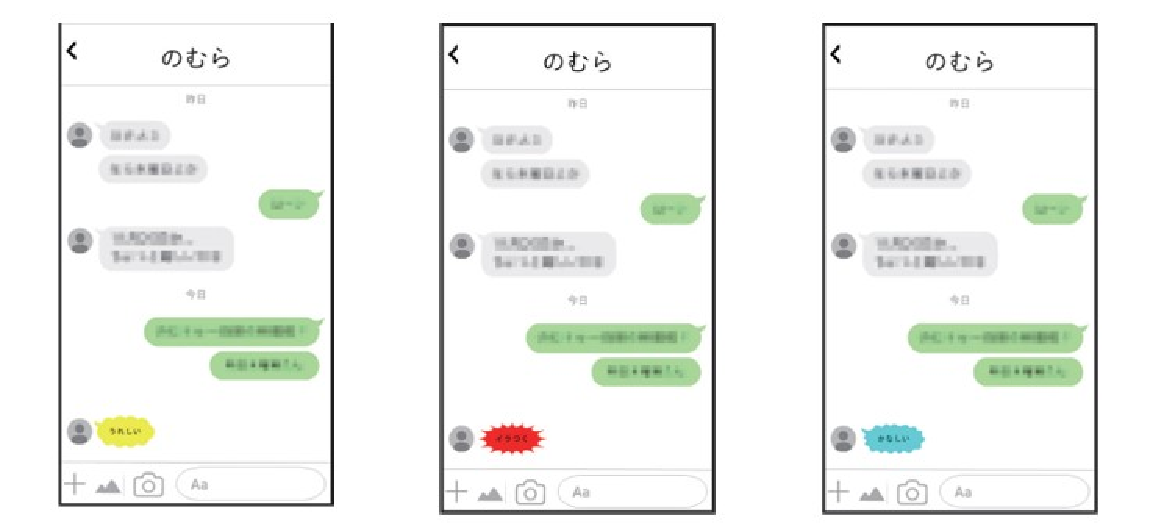
\includegraphics[width=150mm]{PDF/gazou_1.pdf}
        \caption{サンプル画面(左:喜び/サンプル2, 中央:怒り/サンプル6, 右:悲しみ/サンプル4)}
        \label{figure:gazou1}
    \end{center}
\end{figure}

\subsection{音声入力による吹き出しの形状の決定}
青木ら\cite{Thesis_Aoki}は音声入力から感情の覚醒度を検出し、
それに応じた吹き出しを生成する「EmoBalloon」を開発した。
実験の結果、このシステムは送信者と受信者間の感情的認識の一致を向上させることが示された。
現状のテキストチャットでは音声や非言語的手がかりが不足しているため、
テキストチャットにおける感情的覚醒度(emotional arousal)を正確に伝達する方法を提案することを
目的として開発された。日本の漫画データセット「Manga109」を使用し、吹き出しの形状と感情情報を分析し、
吹き出しの形状がメッセージの感情的覚醒度にどのように影響するか調査を行った。
その結果から丸型(中立的な感情)の吹き出しと爆発型
(高覚醒度、怒りなどの強い感情)の吹き出しを利用したチャットシステムを提案した。

% \section{遠距離下でのコミュニケーションツール}
% 本節では遠距離下でのコミュニケーションツールに関する研究について述べる。

% \subsection{遠距離恋愛者間でのコミュニケーション支援ツール}
% 辻田らは遠距離恋愛者間でのコミュニケーションを支援することを目的とした日用品“SyncDecor”を提案した。
% SyncDecorは遠隔地に設置した家具家電の動きを連動させることで両者の生活空間の行為を伝え、
% 仮想的に同居感覚を提供するシステムである。様々な通信手段があるにもかかわらず、
% 遠距離恋愛で悩むカップルが多いことから、
% 両者の生活空間での行為自体が相互に影響を与え合うことを目的とし作成された。
% この研究ではランプの点灯やごみ箱の開閉などを連動させた。
% 例えば片方の家でランプが点灯すればもう片方の家でもランプが点灯するといったシステムになっている。
% 3組のカップルに対し3か月間の実証実験を行ったところ積極的なコミュニケーションツールとして活用され、
% 電話やメールを行うきっかけづくりとなったと述べられている。

\section{本研究の立ち位置}

% \section{本研究の位置づけ}
% 近年のメッセージアプリやメールにおいて、初期の段階で直面していた主なコミュニケーション上の問題は、
% 非言語情報の伝達が限定的であり、それに伴う合意形成の難しさである。
% テキストベースのやり取りでは感情や態度などの微細なニュアンスが伝わりにくく、
% 相手との共感や理解が制約されることがある。
% この問題に対処するため、従来のコミュニケーションツールではスタンプやリアクションといった手段が提供されている。
% これらの機能は、特定の感情や反応をアイコンや絵文字で表現し、
% ユーザー同士のコミュニケーションを豊かにする役割を果たしている。

% 以下図〇はオンラインでコミュニケーションを行うサービス内で、非言語情報を伝える機能をマッピングしたものである。
% 本研究における提案ツールはスタンプやリアクションに比べ記号やイラストといった要素がなく、
% お互いにインタラクションし合う機能が加わったものになる。より効果的な非言語情報の伝達手段として、
% ユーザー間のコミュニケーションの質を向上させることを目的としている。



\chapter{チャットの吹き出しに触れ合う機能の開発と評価}

\section{予備調査}

\subsection{予備調査 概要}
LINEに搭載されているスタンプやリアクション機能といった既存ツールについての調査を
大学・大学院生19名に行った。
普段からLINE等のメッセージアプリのリアクション機能やスタンプ機能を使用しているか、
その使用状況などについて調査した。
また使用した際に自分の感情を表現できているか、自分の感情が相手に伝わっていると感じるか、
相手の感情か伝わってくると感じるかの質問項目について以下にまとめた。
回答は10段階評価を用いた。表現できている・伝わっているが10、
表現できていない・伝わっていないを0として回答を行ってもらった。\\
本予備調査は2024年7月8日から2024年7月10日の間実施した。
回答はGoogleフォームを使用し、大学・大学院生19名に行った。
なお、本実験で使用したインターネットアンケート画面は本論文の付録Aに示すとおりである。

\subsection{目的}
予備調査では、提案ツールの開発にあたり、メッセージアプリにおいて感情表現を行う機能である、
スタンプ機能とリアクション機能に対する使用状況を調査することを目的とする。
また使用状況に加え、メッセージアプリに搭載されている機能が感情表現を行うツールとして効果的かを調査した。

\subsection{質問項目}
表\ref{table:Yobi_tyousa_sitsumon}に質問項目と回答方式を示す。

\vspace{\baselineskip} % 1行分のスペースを挿入
\begin{landscape}%表を90度回転させたい時にこれで囲む
\begin{table}[!ph]
    \caption{LINEのリアクション・スタンプ機能の使用に関する調査アンケート}
    \label{table:Yobi_tyousa_sitsumon}
    \vspace{5mm}
    \centering
    \begin{tabular}{p{1cm}p{10cm}p{8.5cm}} % 列幅を指定して長い内容を改行
        \bhline
         & 質問項目 & 回答方法  \\
        \hline
        Q1 &メッセージアプリ(LINE等)のリアクション機能やスタンプ機能を使用しますか   
           & 選択式(リアクション・スタンプ機能ともによく使う/
           リアクション・スタンプ機能ともにたまに使う/
           リアクション機能のみよく使う/
           リアクション機能のみたまに使う/
           スタンプ機能のみよく使う/
           スタンプ機能のみたまに使う/
           どちらもほとんど使わない) \\
        Q2 &メッセージアプリ(LINE等)のリアクション機能やスタンプ機能を使用するときはどんな時ですか (複数回答可) 
           & 選択式(相手の話に対する自分のリアクションを伝えたいとき/
           会話を終わらせたいとき/
           既読を相手に伝えるため/
           うまい返信を考えつかないとき/
           すぐに返事をできないとき)・自由回答 \\
        Q3 &リアクション・スタンプ機能を使用する際、自分の感情を表現できていると感じるか    
            & 10段階評価(1:表現できていない~10:表現できている) \\
        Q4 &リアクション・スタンプ機能を使用する際、自分の感情が相手に伝わっていると感じるか    
            & 10段階評価(1:伝わっていない~10:伝わっている) \\
        Q5 &相手がリアクション・スタンプ機能を使用した際、相手の感情が伝わってくると感じるか    
            & 10段階評価(1:伝わってこない~10:伝わってくる) \\
        \hline
    \end{tabular}
    \vspace{1cm} % 表との間隔を調整
    \parbox{1.0\textwidth}{\small ※Q2~Q4はQ1にて使用すると答えた場合のみ回答}
\end{table}
\end{landscape}

\subsection{アンケート結果}
Q1のメッセージアプリのリアクション機能やスタンプ機能の使用状況に対しては、約95%が
「リアクション・スタンプ機能ともによく使う」という回答であった。また、Q2の
メッセージアプリのリアクション機能やスタンプ機能を使用する状況に対しての回答結果を図\ref{figure:graph1}に示す。

\vspace{\baselineskip} % 1行分のスペースを挿入
\begin{figure}[htbp]
    \begin{center}
        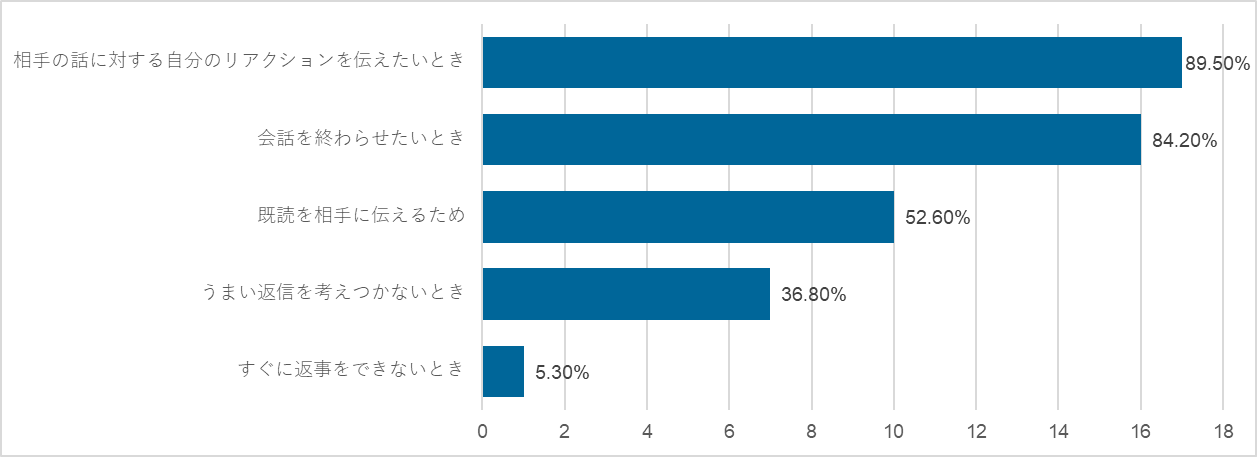
\includegraphics[width=100mm]{PDF/graph_1.png}
        \caption{Q2 回答結果}
        \label{figure:graph1}
    \end{center}
\end{figure}

% 「相手に対する自分のリアクションを伝えたいとき」や「会話を終わらせたいとき」に使用するといった回答が多くみられた。

表\ref{table:Yobi_tyousa_kekka}にQ3からQ5までのアンケート結果を示す。
この結果から、LINEのリアクション・スタンプ機能はユーザー間の感情を伝え合うツールとして有効であるといえる。
これはスタンプやリアクションといったツールは感情を直接的に表すイラストが用いられているため、
ユーザー自身が感じている感情を端的に選ぶことができるからであると考えられる。
本研究では提案ツールを使用することでリアクション機能やスタンプ機能と比較しより微細な感情や、
会話中に生じる体をつついたり、軽くツッコミを入れたりするような表現が可能かどうかを検証を行う。

\vspace{\baselineskip} % 1行分のスペースを挿入
\begin{table}[!ph]
    \caption{LINEのリアクション・スタンプ機能の使用に関する調査アンケート結果}
    \label{table:Yobi_tyousa_kekka}
    \vspace{5mm}
    \centering
    \begin{tabular}{llll}
        \bhline
        項目                   &平均値  \\
        \hline
        自分の感情を表現できていると感じるか   & 7.82 \\
        自分の感情が相手に伝わっていると感じるか & 7.36 \\
        相手の感情が伝わってくると感じるか    & 6.89 \\
        \hline
    \end{tabular}
    \vspace{1cm} % 表との間隔を調整
    \parbox{0.55\textwidth}{\small ※小数点第3位以下は切り捨て}
\end{table}


\section{実験で使用するアプリケーション}
本研究で開発されたメッセージアプリは、既存のメッセージアプリにおける機能を拡張し、
非言語情報の伝達をより効果的に行うための手法を提案し、その有効性を評価することを目的としている。
既存のメッセージアプリで利用可能な非言語情報の表現手段は、感情を表現するイラストや絵文字、
ジェスチャーなどに限られており、その効果的な活用にはさらなる検討が必要であると考えられる。
また、既存のテキストコミュニケーションを行うサービスでは
リアルタイムにインタラクトするような機能が搭載されている事例はあまり無い。
そのため、メッセージアプリで表示される吹き出しに対し、インタラクティブな機能を搭載したメッセージアプリを開発し
実験を行い評価した。

\subsection{プロトタイプの評価}
本研究では、日本で最も使用されているメッセージアプリであるLINEとの比較評価を行うため、
プロトタイプのUIデザインをLINEに似せて設計した。最初に作成したプロトタイプは、
筑波大学の学部生・大学院生4名(2組、各組2人)を対象に予備実験を実施し、使用感を確認した。\\

予備実験の結果、以下の課題が明らかとなった。
\begin{itemize}
    \item 吹き出しの色:LINE上で表示される吹き出しと同じカラー(カラーコード #XXXXXX)を使用していたが、
          アニメーションが見えにくいとの指摘があった。
    \item バイブレーションの長さ:振動時間が長く、通知音のように感じられるとの意見が寄せられた。
\end{itemize}

これらの課題を踏まえ、本実験で使用するメッセージアプリのプロトタイプには以下の変更を加えた。

\begin{itemize}
    \item 吹き出しの色を薄い緑色(カラーコード #XXXXXX)に変更し、アニメーションがより視認しやすいデザインとした。
    \item バイブレーションの時間を短縮し、通知音のように感じられないよう調整を行った。
\end{itemize}

これらの変更により、プロトタイプの視認性や使用感を向上させ、より実験に適したメッセージアプリとして設計を完成させた。
\\
\\
(アプリの変更箇所が分かるような画像)\\
% \begin{figure}[htbp]
%     \begin{center}
%         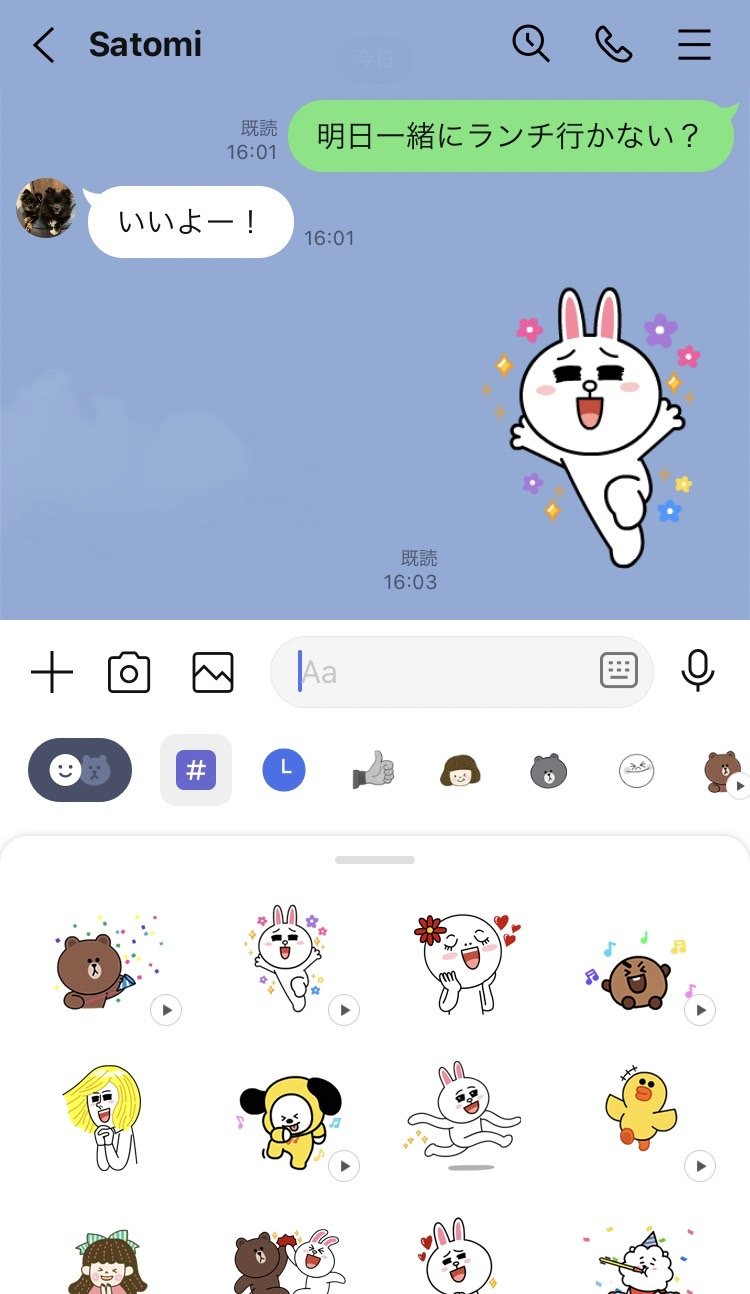
\includegraphics[width=50mm]{PDF/LINE_stamp.jpg}
%         \caption{LINEのスタンプ機能}
%         \label{figure:LINE_stamp}
%     \end{center}
% \end{figure}

\subsection{実験で使用するアプリケーションの仕様}
本研究では、相手の吹き出しに触れるという新しいコミュニケーション機能を導入し、
会話中に生じる触れ合いの感覚を再現可能かどうかを検証することを目的としたメッセージアプリを開発した。
このアプリの開発には、以下の技術を使用した。

\begin{itemize}
    \item フロントエンド: JavaScriptライブラリのPixi.jsを利用し、アニメーションを実現した。
    スプライトシートの作成にはTexturePackerを用いた。
    \item サーバーサイド: Node.jsとSocket.IOを組み合わせ、リアルタイムの通信機能を実現した。
\end{itemize}

作成したアプリケーションは、本実験で使用することを想定し、一対一のコミュニケーションを前提に設計された。
システムの構成図を図\ref{figure:system}に示す。
Webブラウザ上でのメッセージ送受信を前提とし、基本的なメッセージ機能に加えて以下の特徴を備えている。

\begin{itemize}
    \item 吹き出しへの触れ合いアニメーション:
    相手の吹き出しに触れると振動が伝わるようなアニメーションが再生される。
    この機能は、相手側のメッセージに対するリアクションとして設計されており、
    自分のメッセージには反応しない仕組みとなっている。
    \item アニメーションの同期再生:
    吹き出しに触れると、双方の画面でアニメーションが同時に再生される。
    \item 振動フィードバック:
    実験時にキーボードが表示されている場合、画面上部のメッセージが見えなくなる問題を補うため、
    アニメーション再生時にバイブレーションが作動する機能を実装した。
\end{itemize}

本提案ツールは、これらの機能を通じて、従来のテキストベースのメッセージングシステムにはない
新しい触覚的インタラクションの可能性を検証することを目的としている。

システムの動作フローは以下の通りである。\\
1. ユーザーがメッセージを入力し「送信」ボタンをクリック\\
2. メッセージを送信し吹き出しを画面上に表示\\
3. メッセージがサーバーに送信される。\\
4. サーバーは、他のクライアントにメッセージをブロードキャスト\\
5. 各クライアントがメッセージを受信して吹き出しを表示\\
6. 吹き出しをクリックするとクリックイベントがサーバーに送信される\\
7. 他のクライアントにアニメーションイベントがブロードキャストされる

\begin{figure}[htbp]
    \begin{center}
        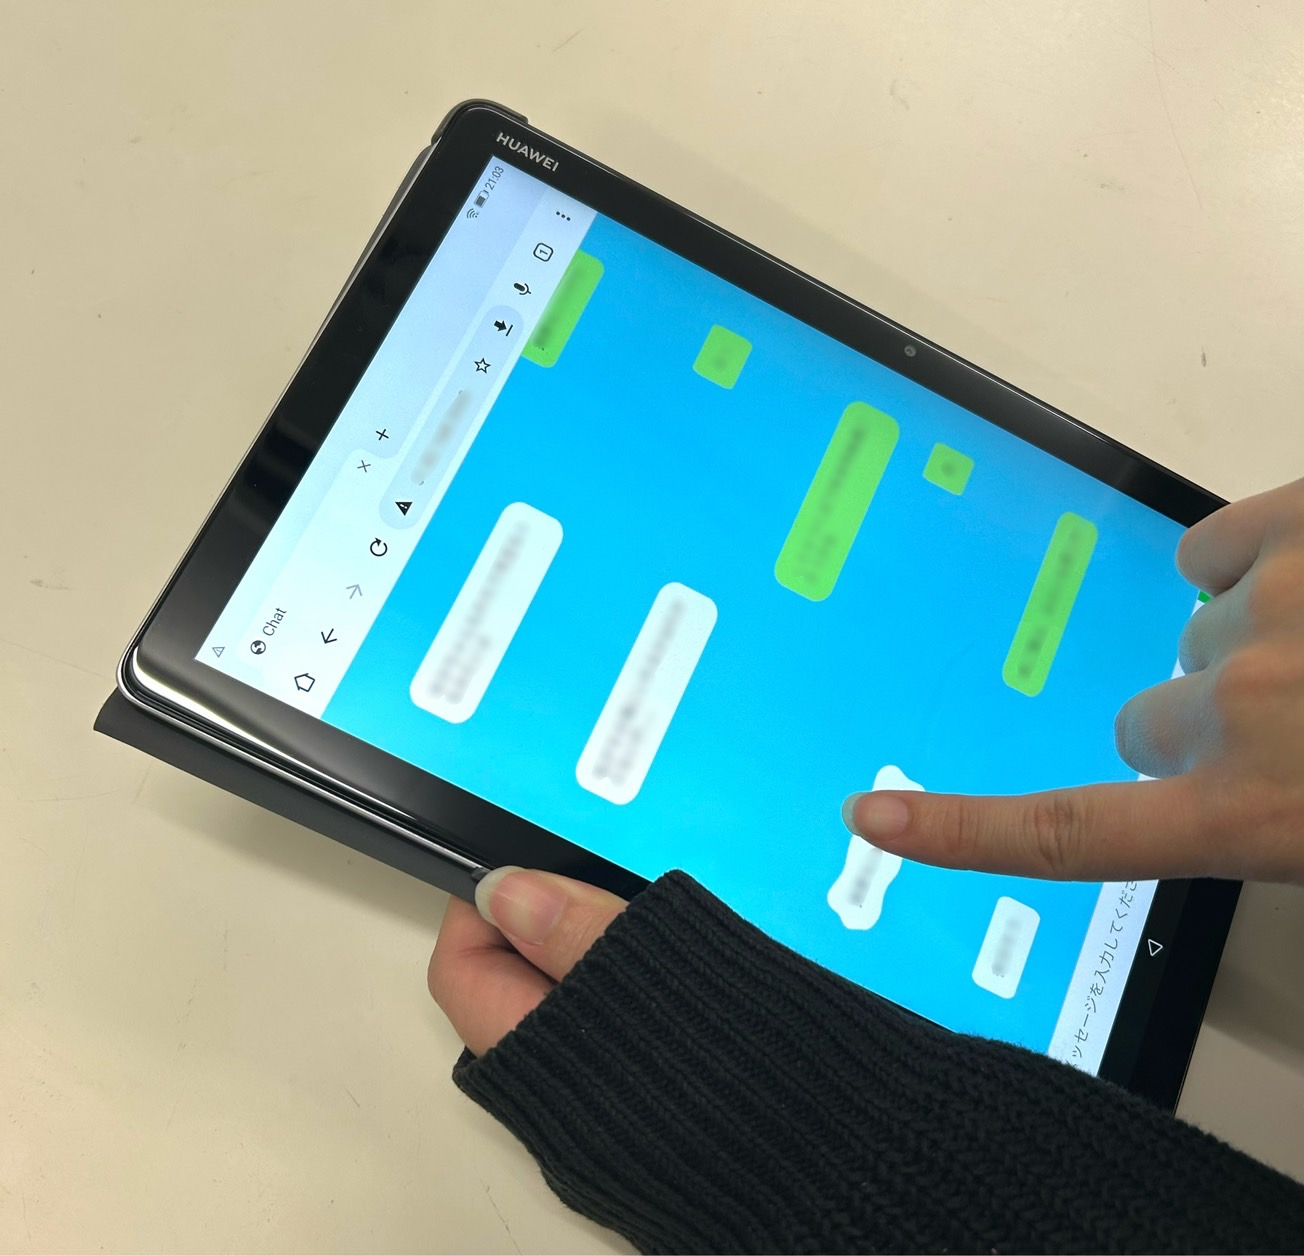
\includegraphics[width=100mm]{PDF/zikken_gamen.jpg}
        \caption{吹き出しに触れるとアニメーションが再生される様子}
        \label{figure:zikken_gamen}
    \end{center}
\end{figure}

\begin{figure}[htbp]
    \begin{center}
        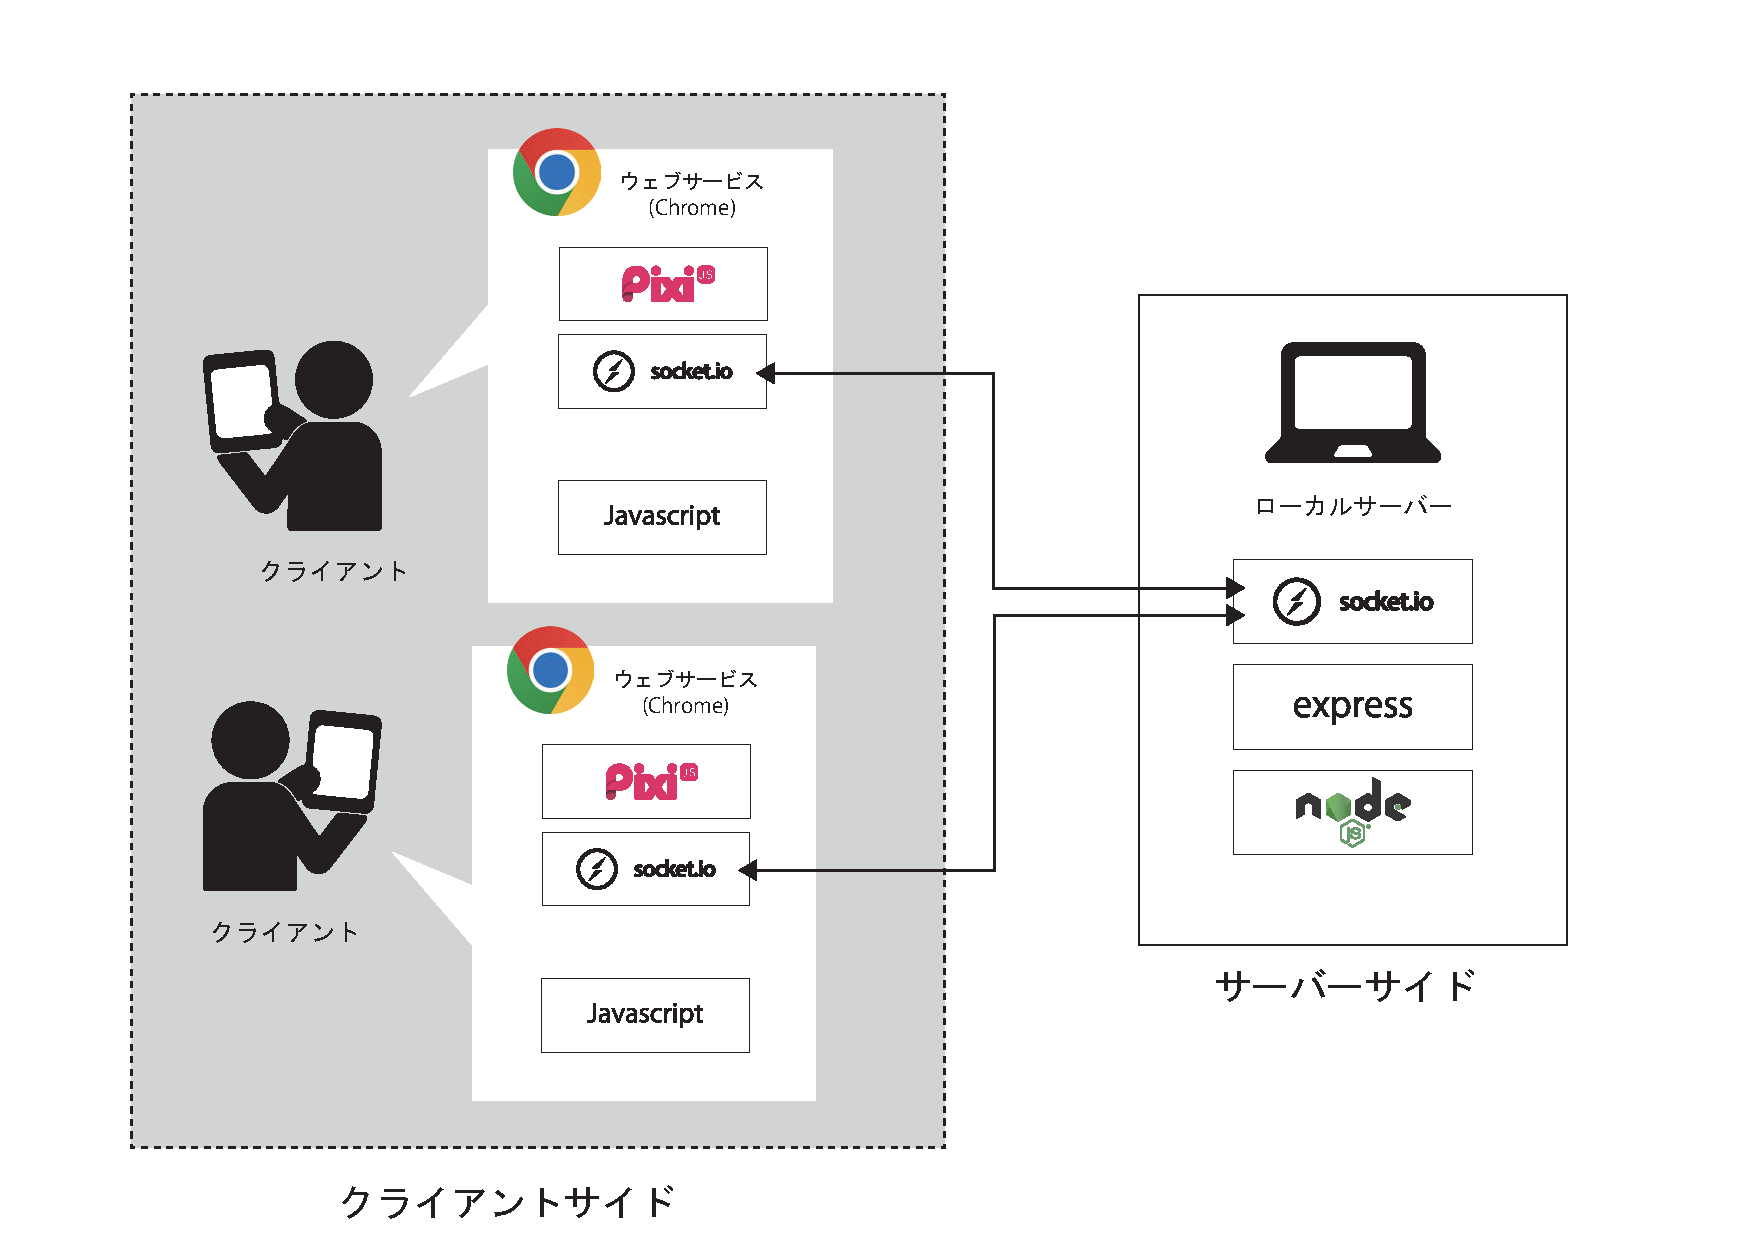
\includegraphics[width=150mm]{PDF/system_2.pdf}
        \caption{実験で使用するアプリケーションのシステム構成図}
        \label{figure:system}
    \end{center}
\end{figure}


\section{実験}

\subsection{概要}
本実験では相手の吹き出しに触れるといったコミュニケーション機能を使用した際に、
会話中に生じるような触れ合いが表現可能かを検証することを目的とする。実験では提案ツールを使用することで、
相手に触れられた感覚(小突く・ツッコミ・つつく)がするか、また触れた際の感情の変化を調査する。
実験は2人ずつ行い、5分の間自由にツールを使用してコミュニケーションを行ってもらう。
その際、
また、このような機能が実装された場合また使用したいと感じるかを調査した。

\subsection{実験環境}
筑波大学の総合研究棟D414室、D518を実験実施場所として使用する(図\ref{figure:D414}、\ref{figure:D518})。

\begin{figure}[htbp]
    \begin{center}
        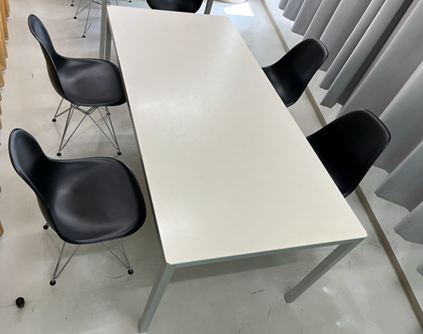
\includegraphics[width=100mm]{PDF/D414.png}
        \caption{総合研究棟D414室}
        \label{figure:D414}
    \end{center}
\end{figure}

\begin{figure}[htbp]
    \begin{center}
        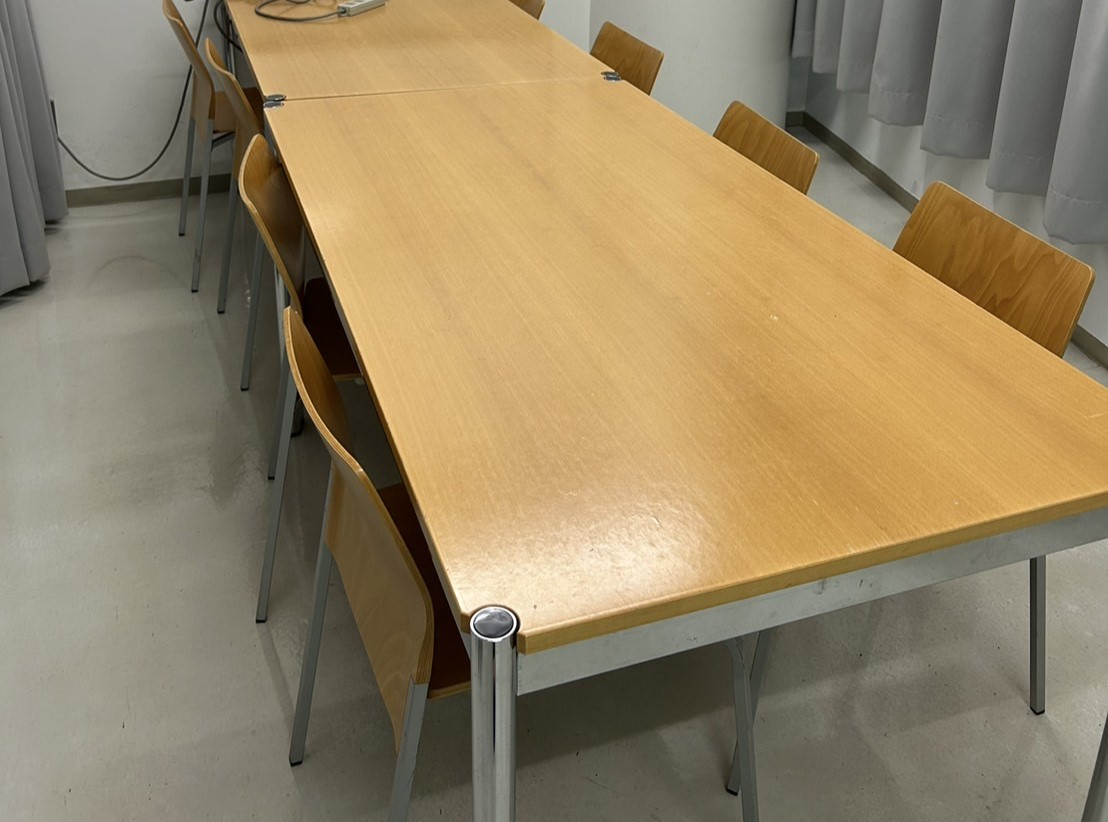
\includegraphics[width=100mm]{PDF/D518.jpg}
        \caption{総合研究棟D518室}
        \label{figure:D518}
    \end{center}
\end{figure}

実験参加者が到着した後、椅子に着席してもらい、実験説明・実施等を行う。
部屋は遮光カーテンを閉めて部屋の照明をつけた状態とする。
実験参加者は図\ref{figure:zikke_kankyo}のような環境で実験を行う。

\begin{figure}[htbp]
    \begin{center}
        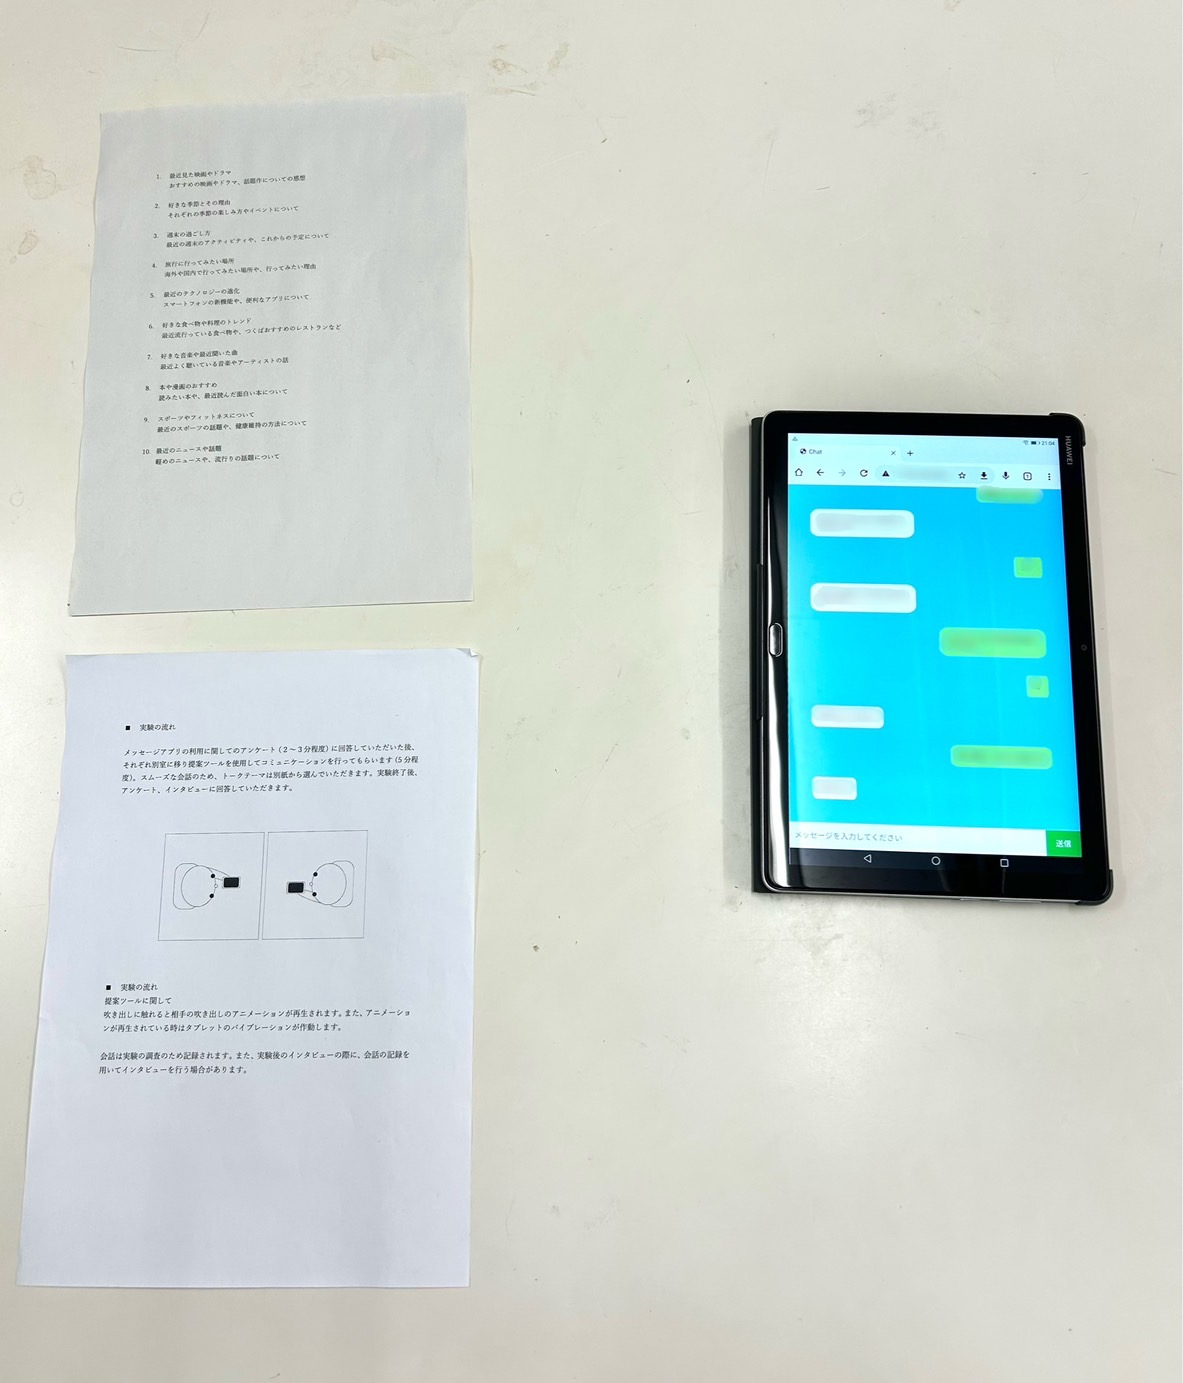
\includegraphics[width=100mm]{PDF/zikke_kankyo.jpg}
        \caption{実験環境}
        \label{figure:zikke_kankyo}
    \end{center}
\end{figure}

実験についての説明後、実験参加者にはタブレットを渡し1人に別室に移ってもらった後、
5分間メッセージアプリを使用して会話を行ってもらう。
タブレットは10.1型HUAWEI MediaPad M5 lite、
アプリケーションを表示するブラウザはGoogle Chromeを使用した。

\subsection{実験手順}
本実験では、以下の手順に基づいて実施した。\\
1.  実験説明と参加同意の確認\\
まず、実験協力者に対して実験の概要を口頭で説明した後、
実験の流れや注意事項が記載された資料を用いて、実験で使用するメッセージアプリの操作方法を
実演しながら説明を行う。その後、説明を十分に理解した上で問題がない場合は、
実験参加に関する同意書にサインをしてもらい、参加同意を得る。\\
2.  実験前アンケート\\
参加同意後、協力者が普段利用しているLINEにおけるスタンプ機能やリアクション機能の使用状況、
さらにそれらを用いた感情表現がうまく行えているかについて尋ねるアンケートを実施する。
アンケートは質問用紙を用いて行う。\\
3.  実験用メッセージアプリの使用\\
アンケート終了後、再度メッセージアプリの操作方法を説明し、
会話をスムーズに進めるための10項目のトークテーマを提示して、その中から1つを選択してもらう。
この際、実験データを収集するため、メッセージアプリ内での会話内容を記録する旨も伝える。
その後、2名の協力者のうち1名に別室へ移動してもらい、
5分間メッセージアプリを使用してコミュニケーションを行った。実験に使用したメッセージアプリには、
相手の吹き出しに触れると振動が伝わるアニメーションが再生される機能が搭載されている。
また、タブレットのキーボード表示時に画面上部のメッセージが見えなくなる可能性を考慮し、
アニメーション再生時にバイブレーションが作動する機能も付加されている。
このため、協力者にはタブレットを持った状態で実験を行うよう説明する。\\
4.  実験後アンケート\\
実験終了後、実験で使用したメッセージアプリの機能に関する感想や意見を尋ねるアンケートを実施する。
アンケートは質問用紙を用いて行う。\\
5.  インタビュー\\
アンケート終了後、協力者へのインタビューを行い、実験全体の感想や意見を聞く。
その後、全ての実験手順を終了する。\\

\begin{figure}[htbp]
    \begin{center}
        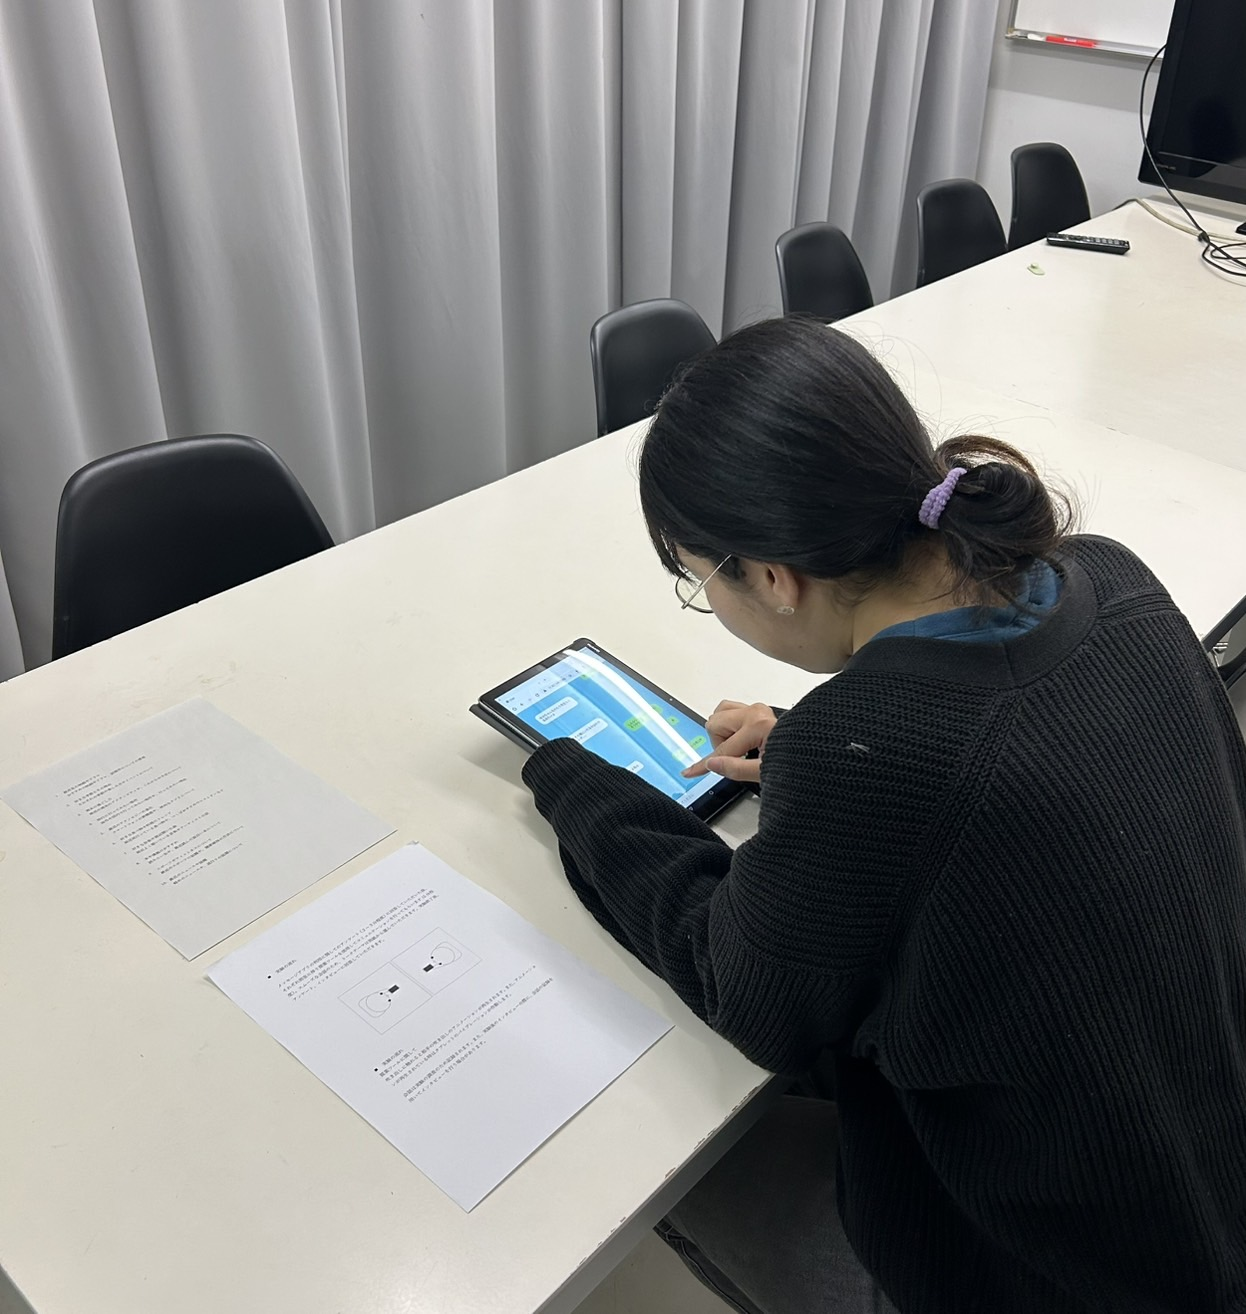
\includegraphics[width=100mm]{PDF/zikken_yousu.jpg}
        \caption{実験の様子}
        \label{figure:zikken_yousu}
    \end{center}
\end{figure}

\subsection{評価項目}
表\ref{table:zikken_sitsumon}に質問項目を示す。
評価にはVAS法(Visual Analog Scale)を使用した\cite{Thesis_Takahashi1}\cite{Thesis_Takahashi2}。
VAS法とは視覚的アナログ尺度と訳され、痛みなどを客観的に評価するために「無痛」から「最強の苦痛」までの表現を
線分上に回答する方法である\cite{Thesis_vas}。今回は左端を「全く○○ではなかった」、
右端を「非常に○○だった」などとする100mmの線分(回答用線分)上の任意のポイントを被験者に手書きで線を入れてもらった。
そして、左端から縦線までの長さを10点満点に換算した。 
自覚的な心理量測定には,一般的に段階尺度による評定法または量推定法が用いられることが多いが、
VAS法は評価のステップ幅を被験者任せにするという点で後者に近い性質をもっている。
本研究では「集団平均値の変動」だけでなく「個人内変動」も問題にしている。
微細な個人内変動をデータ化することに意味があるといった観点から、段階尺度よりは量推定法の方が有効と考えられた。
さらに、同一の調査を二度繰り返すという手続きには不可避的に記憶実験的な要素が入り込むため、
具体的な数値を表出させる量推定法よりもその点を曖昧にしたアナログ尺度の方がより適切であると判断した。

\vspace{\baselineskip} % 1行分のスペースを挿入
\begin{table}[!ph]
    \caption{実験で使用したメッセージアプリの機能に関する調査アンケート}
    \label{table:zikken_sitsumon}
    \vspace{5mm}
    \centering
    \begin{tabular}{p{1cm}p{12cm}} % 列幅を指定して長い内容を改行
        \bhline
         & 質問項目 \\ % 見出し行を追加
        \hline
        & (相手のメッセージの吹き出しに触れた時のことについて) \\
        Q1 & 自分の感情が表現できたと感じるか \\
        Q2 & 相手に自分の感情が伝わったと思うか \\
        & (相手があなたの吹き出しに触れた時について) \\
        Q3 & 自分自身が触れられたような感覚はあったか \\
        Q4 & 小突かれたような感じがした \\
        Q5 & ツッコミを受けたような感じがした \\
        Q6 & 相手の感情が伝わってきたと感じたか \\
        Q7 & 相手からのアクションに対し同じようにアクションを返したくなるか \\
        & (ツールの使用感に関して) \\
        Q8 & 機能が実装された場合また使用したいか \\
        Q9 & このUIがあなたの普段使用しているメッセージアプリに実装された場合使ってみたいと思うか \\
        \hline
    \end{tabular}
\end{table}

\subsection{結果と分析}
表\ref{table:zikken_kekka}に結果を示す。
メッセージアプリの使用に関する質問項目間の関係性を調べるため、
JASP\cite{book_JASP}を用いて無相関検定を実施した。この分析では、各質問項目間の相関を確認し、関連性があるかどうかを統計的に評価した。
その結果、以下の項目間で0.1%水準で有意な強い正の相関が認められた。

Q1(自分の感情が表現できたと感じるか)とQ2(相手に自分の感情が伝わったと感じるか)\\
相関係数:r = X.XX(p < 0.05)\\

Q1とQ7(つつかれたような感じがしたか)\\
相関係数:r = X.XX(p < 0.05)\\

Q2とQ7\\
相関係数:r = X.XX(p < 0.05)\\

Q3(相手の感情が伝わったと感じるか)とQ4(相手からのアクションに対し同じようにアクションを返したくなるか)\\
相関係数:r = X.XX(p < 0.05)\\

Q3とQ5(小突かれたような感じがしたか)\\
相関係数:r = X.XX(p < 0.05)\\

Q4とQ5\\
相関係数:r = X.XX(p < 0.05)\\

これらの結果は、特定の機能がユーザーの感情表現や相互作用にどのように影響を及ぼすかを示唆している。
特に、アプリのアニメーションや触覚フィードバックが、感情表現や相手とのインタラクションに関連する可能性が示された。
また、Q1とQ7、Q2とQ7の相関は、感情表現と触覚的なフィードバック
(例:つつかれる感覚)が密接に関連していることを示している。
同様に、Q3とQ4、Q3とQ5の相関は、相手の感情が伝わったと感じる要因が、
インタラクションの動機づけや触覚的な体験に関連している可能性を示している。
これらの知見は、提案したメッセージアプリの機能設計が、
感情の伝達とコミュニケーションの質に与える影響を明らかにする重要な手がかりを提供している。

\vspace{\baselineskip} % 1行分のスペースを挿入
\begin{table}[!ph]
    \caption{実験で使用したメッセージアプリの機能に関する調査アンケート結果}
    \label{table:zikken_kekka}
    \vspace{5mm}
    \centering
    \begin{tabular}{p{3cm}p{3cm}p{3cm}} % 列幅を指定して長い内容を改行
        \bhline
        質問項目 & M(平均) & SD(標準偏差) \\ % 見出し行を追加
        \hline
        Q1 & 5.80 & 1.99\\
        Q2 & 5.83 & 2.01\\
        Q3 & 4.99 & 2.46\\
        Q4 & 5.90 & 2.20\\
        Q5 & 5.79 & 2.55\\
        Q6 & 5.01 & 2.32\\
        Q7 & 5.58 & 1.97\\
        Q8 & 7.43 & 1.71\\
        Q9 & 7.83 & 1.58\\
        Q10 \\
        \hline
    \end{tabular}
    \vspace{1cm} % 表との間隔を調整
    \parbox{0.55\textwidth}{\small ※小数点第3位以下は切り捨て}
\end{table}




\chapter{考察}
\subsection{考察}



\chapter{結論}



\pagestyle{fancy}
\fancyhead{} % clear all header fields
\lhead{謝辞} %ヘッダ左
\chead{} %ヘッダ中央
\rhead{\thepage} %ヘッダ右.コンパイルした日付を表示
\lfoot{} %フッタ左
\cfoot{} %フッタ中央.ページ番号を表示
% \rfoot{造形・メディアデザインコース} %フッタ右
\renewcommand{\footrulewidth}{0.5pt} %フッタの罫線


\chapter*{謝辞}
\addcontentsline{toc}{chapter}{謝辞} %謝辞を目次に掲載するための処理
研究及び本論文執筆にあたり、システム案の相談や論文の添削など多方面において助言をして頂きました
芸術系山田博之准教授に深くお礼申し上げます。また芸術系米亜助教には、本論文の作成にあたり、
副査として適切なご助言を賜りました。感謝申し上げます。
さらに、研究を進めるにあたって日常の多くの知識や示唆を頂戴致しました、山田博之研究室の皆様、
アンケートの回答、実験にご協力いただいた筑波大学の先生方と学生の皆様に深くお礼申し上げます。

\newpage
\pagestyle{fancy}
\fancyhead{} % clear all header fields
\lhead{参考文献} %ヘッダ左
% \renewcommand{\chaptermark}[1]{\lhead{第\ \thechapter\ 章~~~#1}{}}
\chead{} %ヘッダ中央
\rhead{\thepage} %ヘッダ右.コンパイルした日付を表示
\lfoot{} %フッタ左
\cfoot{} %フッタ中央.ページ番号を表示
% \rfoot{造形・メディアデザインコース} %フッタ右
\renewcommand{\footrulewidth}{0.5pt} %フッタの罫線

%------参考文献    
\pagestyle{fancy}
\fancyhead{} % clear all header fields
\lhead{参考文献} %ヘッダ左
\renewcommand{\chaptermark}[1]{\lhead{参考文献\ \thechapter\ ~~~#1}{}}
\chead{} %ヘッダ中央
\rhead{\thepage} %ヘッダ右.コンパイルした日付を表示
\lfoot{} %フッタ左
\cfoot{} %フッタ中央.ページ番号を表示
% \rfoot{造形・メディアデザインコース} %フッタ右
\renewcommand{\footrulewidth}{0.5pt} %フッタの罫線
\titleformat{\chapter}[display]{\huge\bfseries}{参考文献\ \thechapter}{20pt}{}[]

\begin{thebibliography}{99} % 参考文献
    \bibitem{book_Susan}
    %  著者: 翻訳本のタイトル, 出版社, ページ数, 発行年.
    Susan R Fussell: Introduction and overview. In The verbal communication of emotions, 
    Psychology Press, 9–24. 2002.

    \bibitem{Web1}
    総務省: 令和5年度 情報通信メディアの利用時間と情報行動に関する調査,
    \url{https://www.soumu.go.jp/iicp/research/results/media_usage-time.html}(参照 2024-12-13).

    \bibitem{Thesis_Joseph}
    Joseph B. Walther: Interpersonal Efects in Computer-Mediated Interaction, 
    Communication Research 19, 1(feb 1992), 52–90, 1992.

    \bibitem{Thesis_Joseph2}
    Joseph B. Walther, Yuhua Liang, David DeAndrea, Stephanie Tong, Caleb Carr, 
    Erin Spottswood, Yair Amichai-Hamburger:
    The Efect of Feedback on Identity Shift in Computer-Mediated Communication, 
    Media Psychology, 14(mar 2011), 1–26, 2011.

    \bibitem{Thesis_Morimoto} 
    % 著者:標題,雑誌名,巻,号,頁,年.
    森本洋一.メッセージングアプリの機能がコミュニケーションにおいて果たす役割に関する一考察,
    専修大学情報科学研究所所報, 86, 19-24, 2016.

    \bibitem{Thesis_Okamoto}
    岡本卓也: SNSストレス尺度の作成とSNS利用動機の違いによるSNSストレス,
    信州大学人文科学論集, 4, 113-131, 2017.

    \bibitem{Thesis_Nomura}
    野村竜成,田村良一: メッセージングアプリケーションにおける感情伝達のための表現方法に関する研究,
    日本感性工学論文誌, 21(3), 309-316, 2022.

    \bibitem{Thesis_Ozawa}
    小澤 賢司, 清水 忍: フェイスマークが伝える感性情報,

    \bibitem{Web2}
    LINEキャンパス: LINEの特徴やユーザーを知る,
    \url{https://campus.line.biz/line-ads/courses/user/lessons/oada-1-2-2}(参照 2024-12-13).

    \bibitem{Web3} %画像の引用元
    LINEみんなの使い方ガイド: より便利になった!スタンプキーボードの使い方,
    \url{https://guide.line.me/ja/stickers-emojis-themes/sticker-keyboard.html}(参照 2024-12-13).

    \bibitem{Thesis_Liu}
    Miki Liu, AustinWong, Ruhi Pudipeddi, Betty Hou, DavidWang, and Gary Hsieh: 
    ReactionBot: Exploring the Efects of Expression-Triggered Emoji in Text Messages, 
    Proceedings of the ACM on Human-Computer Interaction 2, CSCW,
    Article 110 (nov 2018), 1–16, 1018.

    \bibitem{Thesis_Aoki}
    Toshiki Aoki, Rintaro Chujo, Katsufumi Matsui, Saemi Choi, Ari Hautasaari:
    EmoBalloon - Conveying Emotional Arousal in Text Chats with Speech Balloons,
    In CHI Conference on Human Factors in Computing Systems, Article 527(CHI '22), 1–16, 2022.

    \bibitem{Thesis_Takahashi1}
    高橋晋也, 羽成隆司: 色嗜好表出における認知要因, 
    日本色彩学会誌, 29(1), 14-23, 2005.

    \bibitem{Thesis_Takahashi2}
    羽成隆司,高橋晋也: 認知的操作がvisual analog scaleによる色嗜好測定に及ぼす効果:色好嫌の活性化課題を用いて, 
    日本色彩学会誌, 28(0), 48-49, 2004.

    \bibitem{Thesis_vas}
    Timothy H. Monk: A visual analogue scale technique to measure global vigor and affect, 
    Psychiatry Research, 27(1), 89-99, 1989. 

    \bibitem{book_JASP} % 本
    %  著者: 翻訳本のタイトル, 出版社, ページ数, 発行年.
    清水優菜, 山本光:JASPで今すぐ始める統計解析入門 心理・教育・看護・社会系のために, 
    講談社, 160p, 2022.

    % \bibitem{Book2} % 翻訳本
    % %  著者, 翻訳者(訳): 翻訳本のタイトル, 出版社, ページ数, 発行年.
    % ジョゼ・サラマーゴ, 木下 眞穂(訳): 象の旅, 書肆侃侃房, 216p, 2021.

    % \bibitem{Web} % Webサイト
    % %  サイト名:ページ名(オンライン),\url{https://} (参照 2021-12-34).
    % 香川大学:造形・メディアデザインコース(オンライン), \url{https://www.kagawa-u.ac.jp/kagawa-u_ead/course/modeling/} (参照 2021-12-24).

    % \bibitem{Yamamoto} % Webサイト
    % %  サイト名:ページ名(オンライン),\url{https://} (参照 2021-12-34).
    % TDCC LABORATORY:卵形曲線を表す方程式(オンライン), \url{https://nyjp07.com/index_egg.html} (参照 2021-1-10).

\end{thebibliography}
%------ここまで参考文献

%------付録
\newpage
\appendix         % 付録
\pagestyle{fancy}
\fancyhead{} % clear all header fields
% \lhead{付録} %ヘッダ左
\renewcommand{\chaptermark}[1]{\lhead{付録\ \thechapter\ ~~~#1}{}}
\chead{} %ヘッダ中央
\rhead{\thepage} %ヘッダ右.コンパイルした日付を表示
\lfoot{} %フッタ左
\cfoot{} %フッタ中央.ページ番号を表示
% \rfoot{造形・メディアデザインコース} %フッタ右
\renewcommand{\footrulewidth}{0.5pt} %フッタの罫線

\titleformat{\chapter}[display]{\huge\bfseries}{付録\ \thechapter}{20pt}{}[]

\chapter{予備調査 アンケート画面}

\section{インターネットアンケート画面}

\titleformat{\chapter}[display]{\huge\bfseries}{付録\ \thechapter}{20pt}{}[]

\chapter{実験資料}

\section{実験の説明}
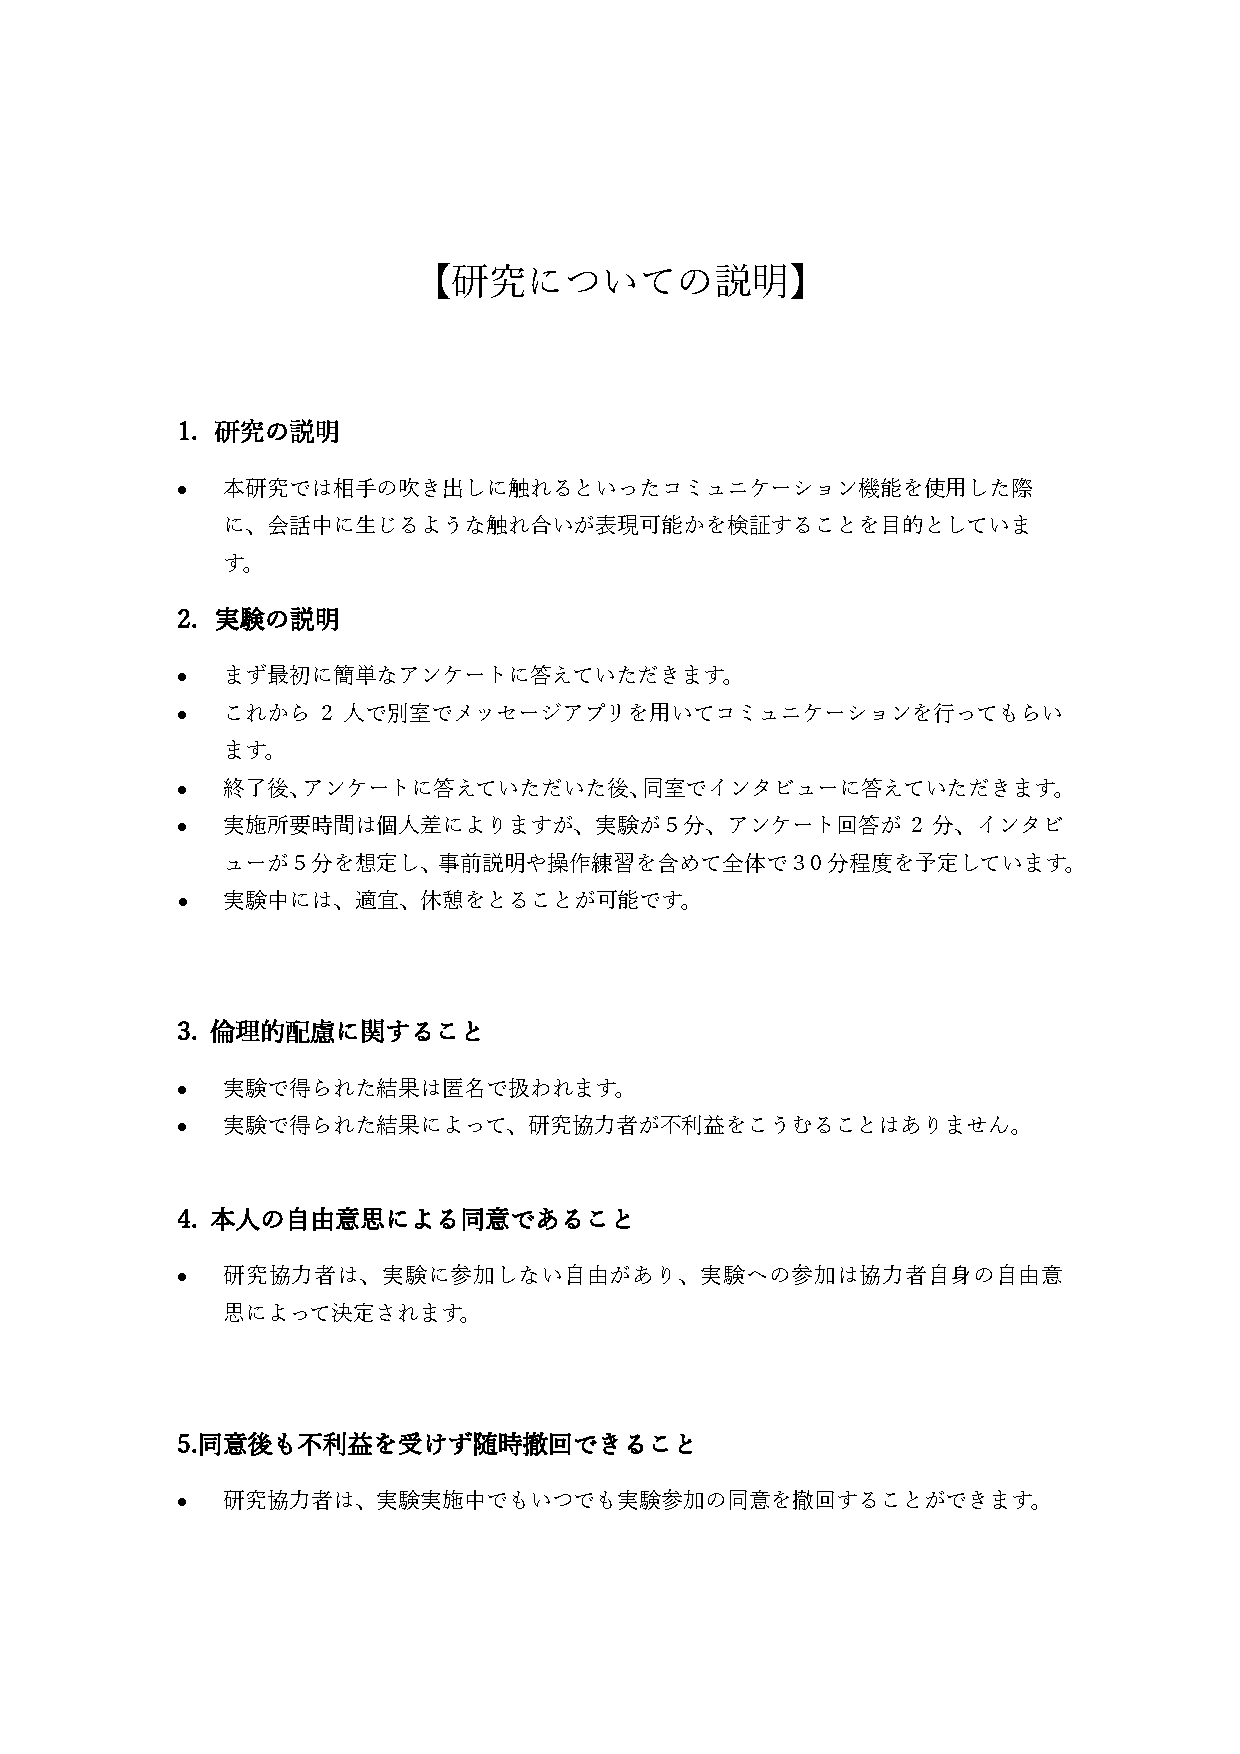
\includepdf[pages=-, scale=0.9]{PDF/setsumei.pdf} % PDFを挿入

\section{実験の説明}
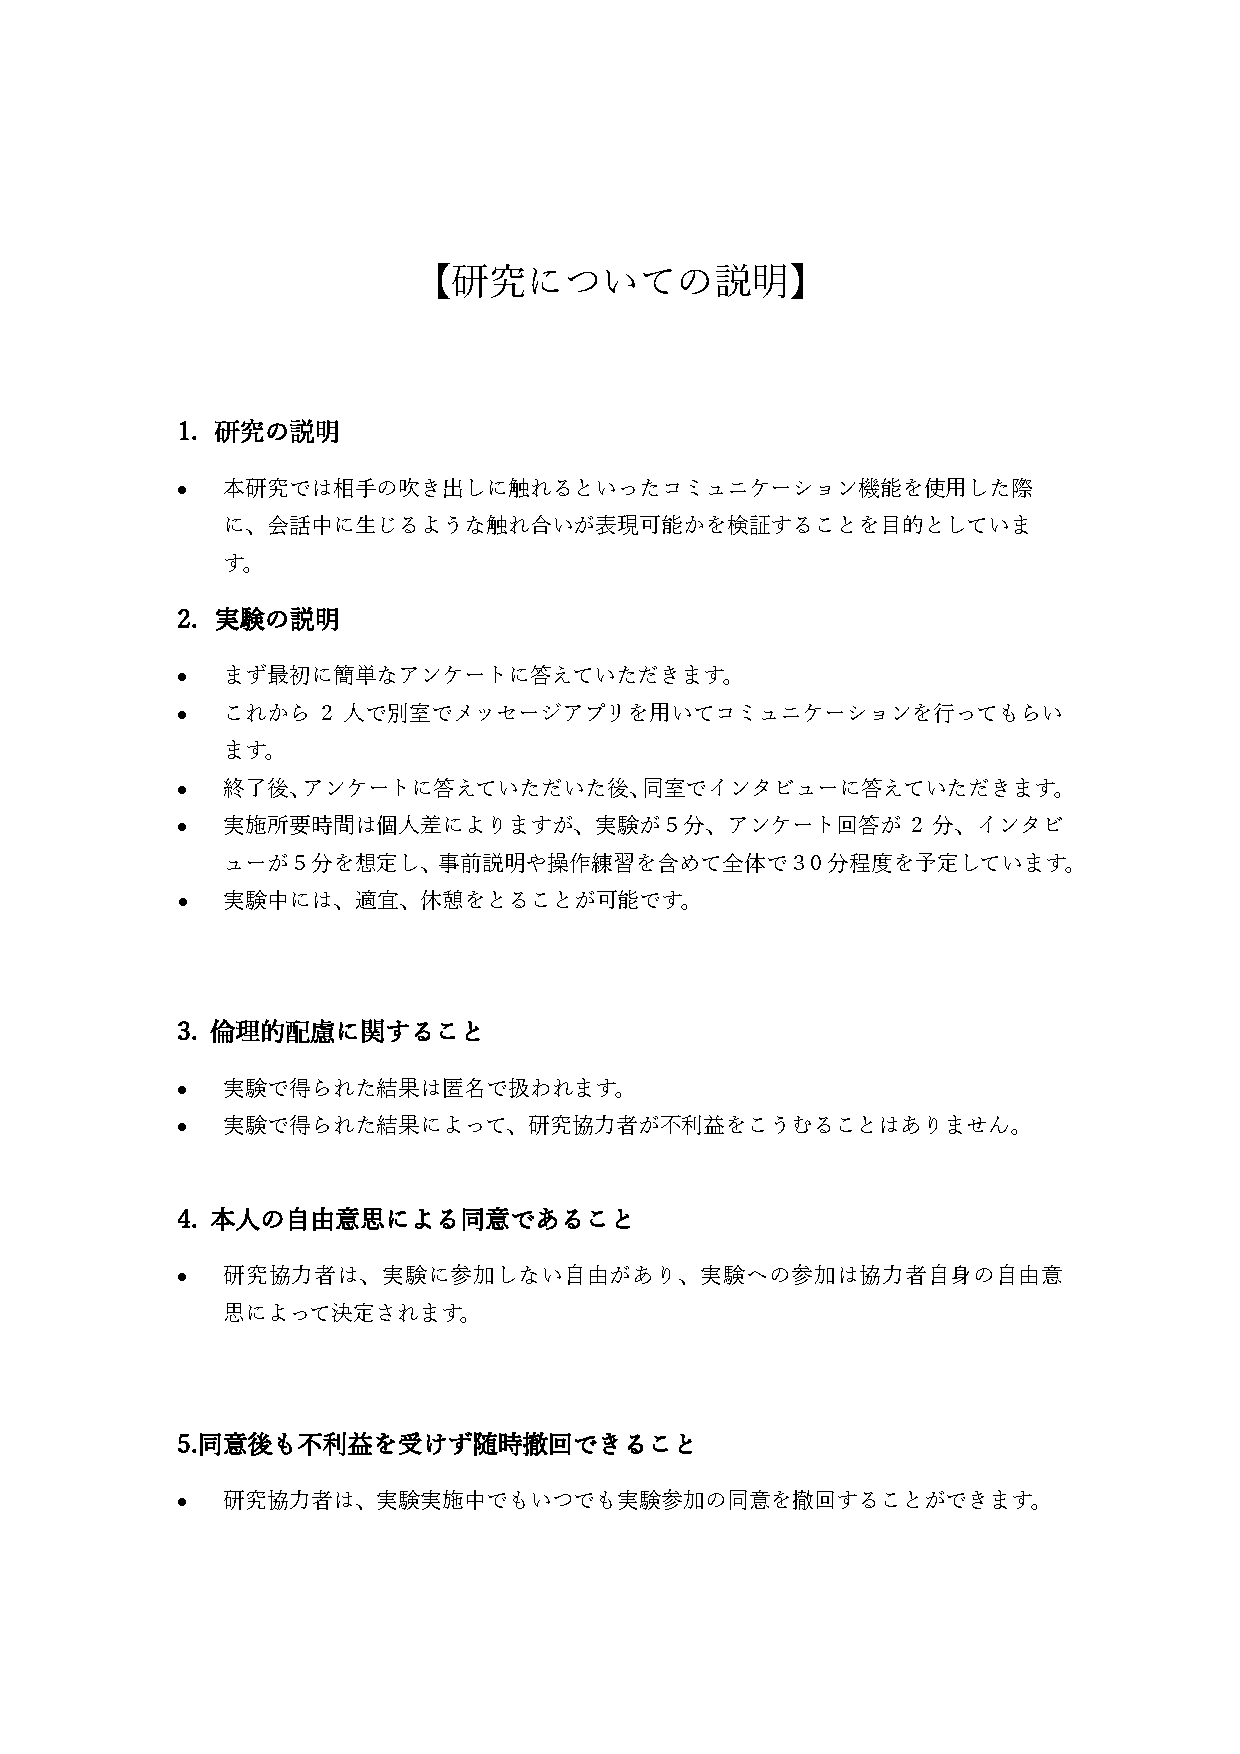
\includepdf[pages=-, scale=0.9]{PDF/setsumei.pdf}

\section{トークテーマ一覧}
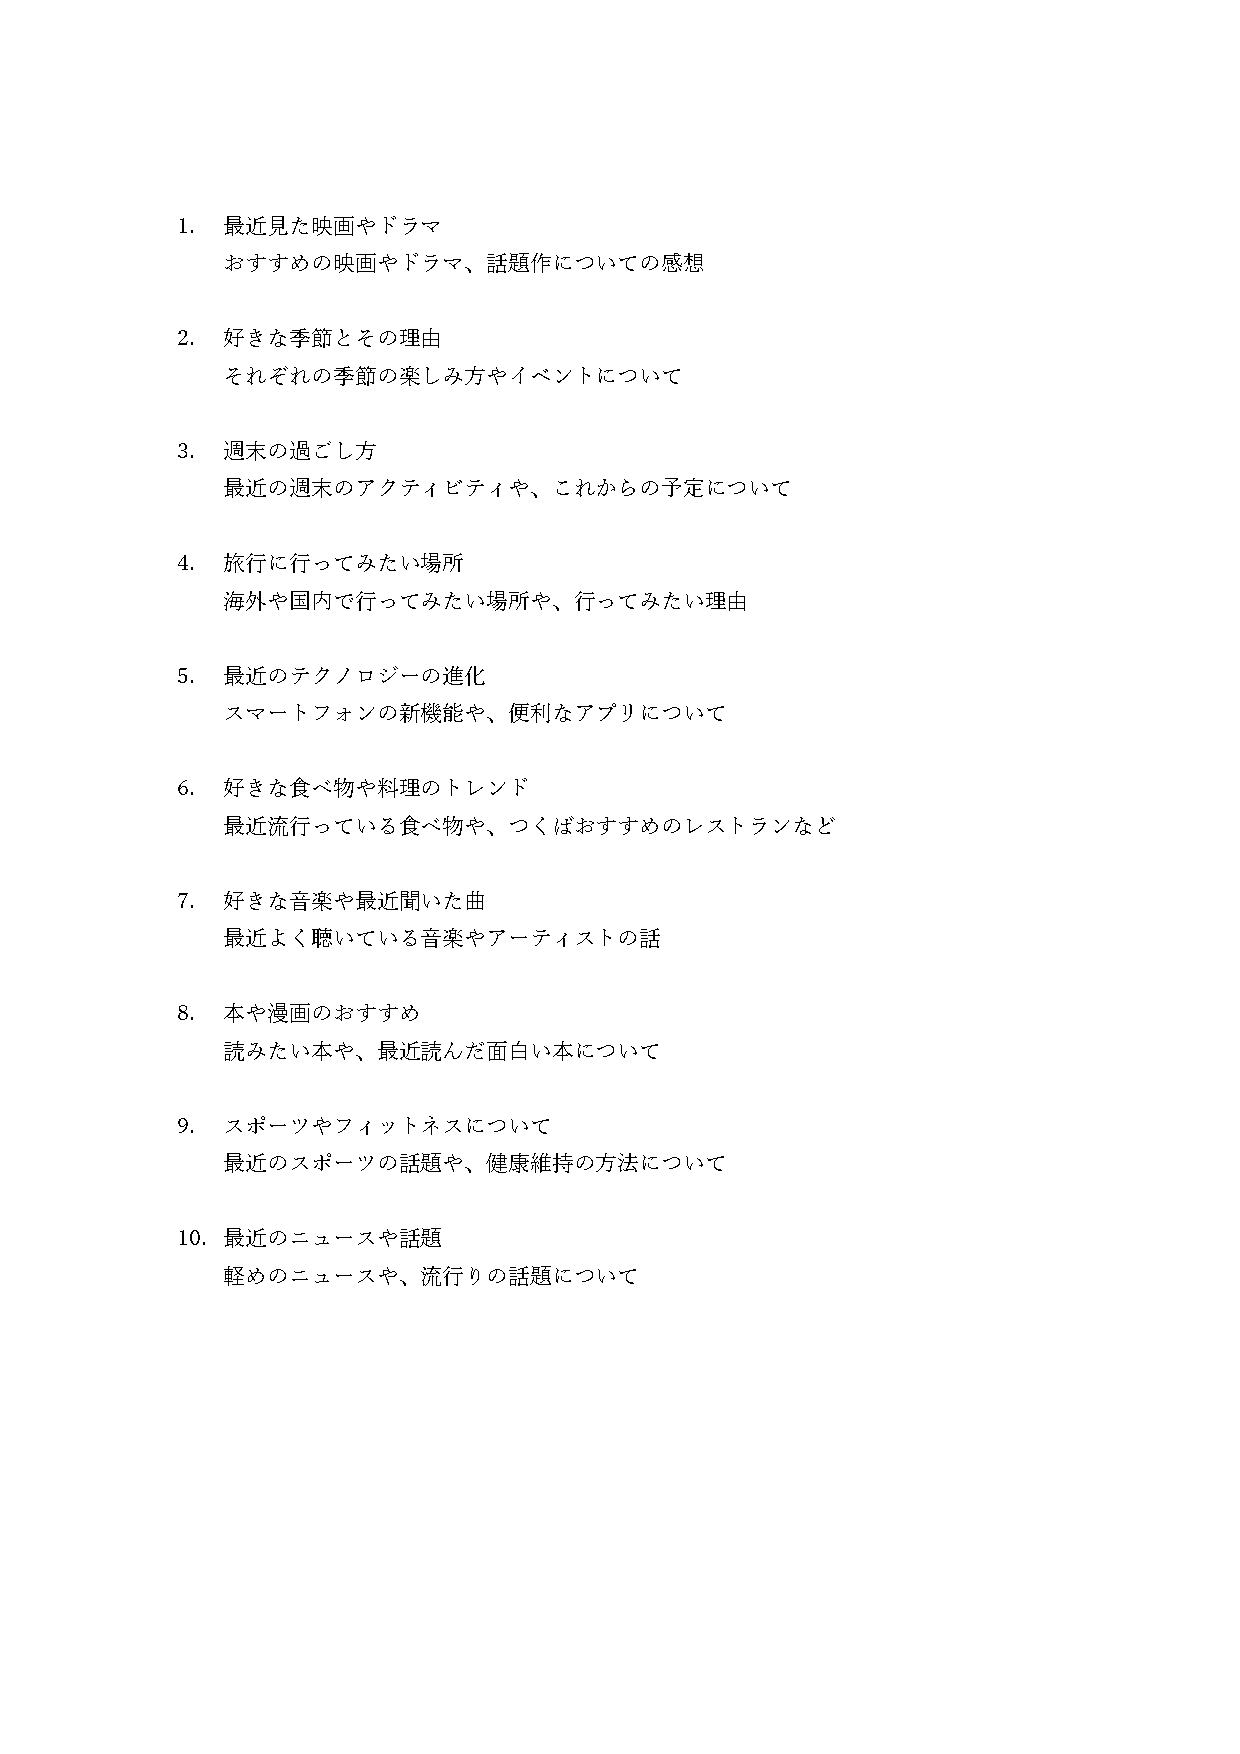
\includepdf[pages=-, scale=0.9]{PDF/talk_thema_ja.pdf}

\section{アンケート①}
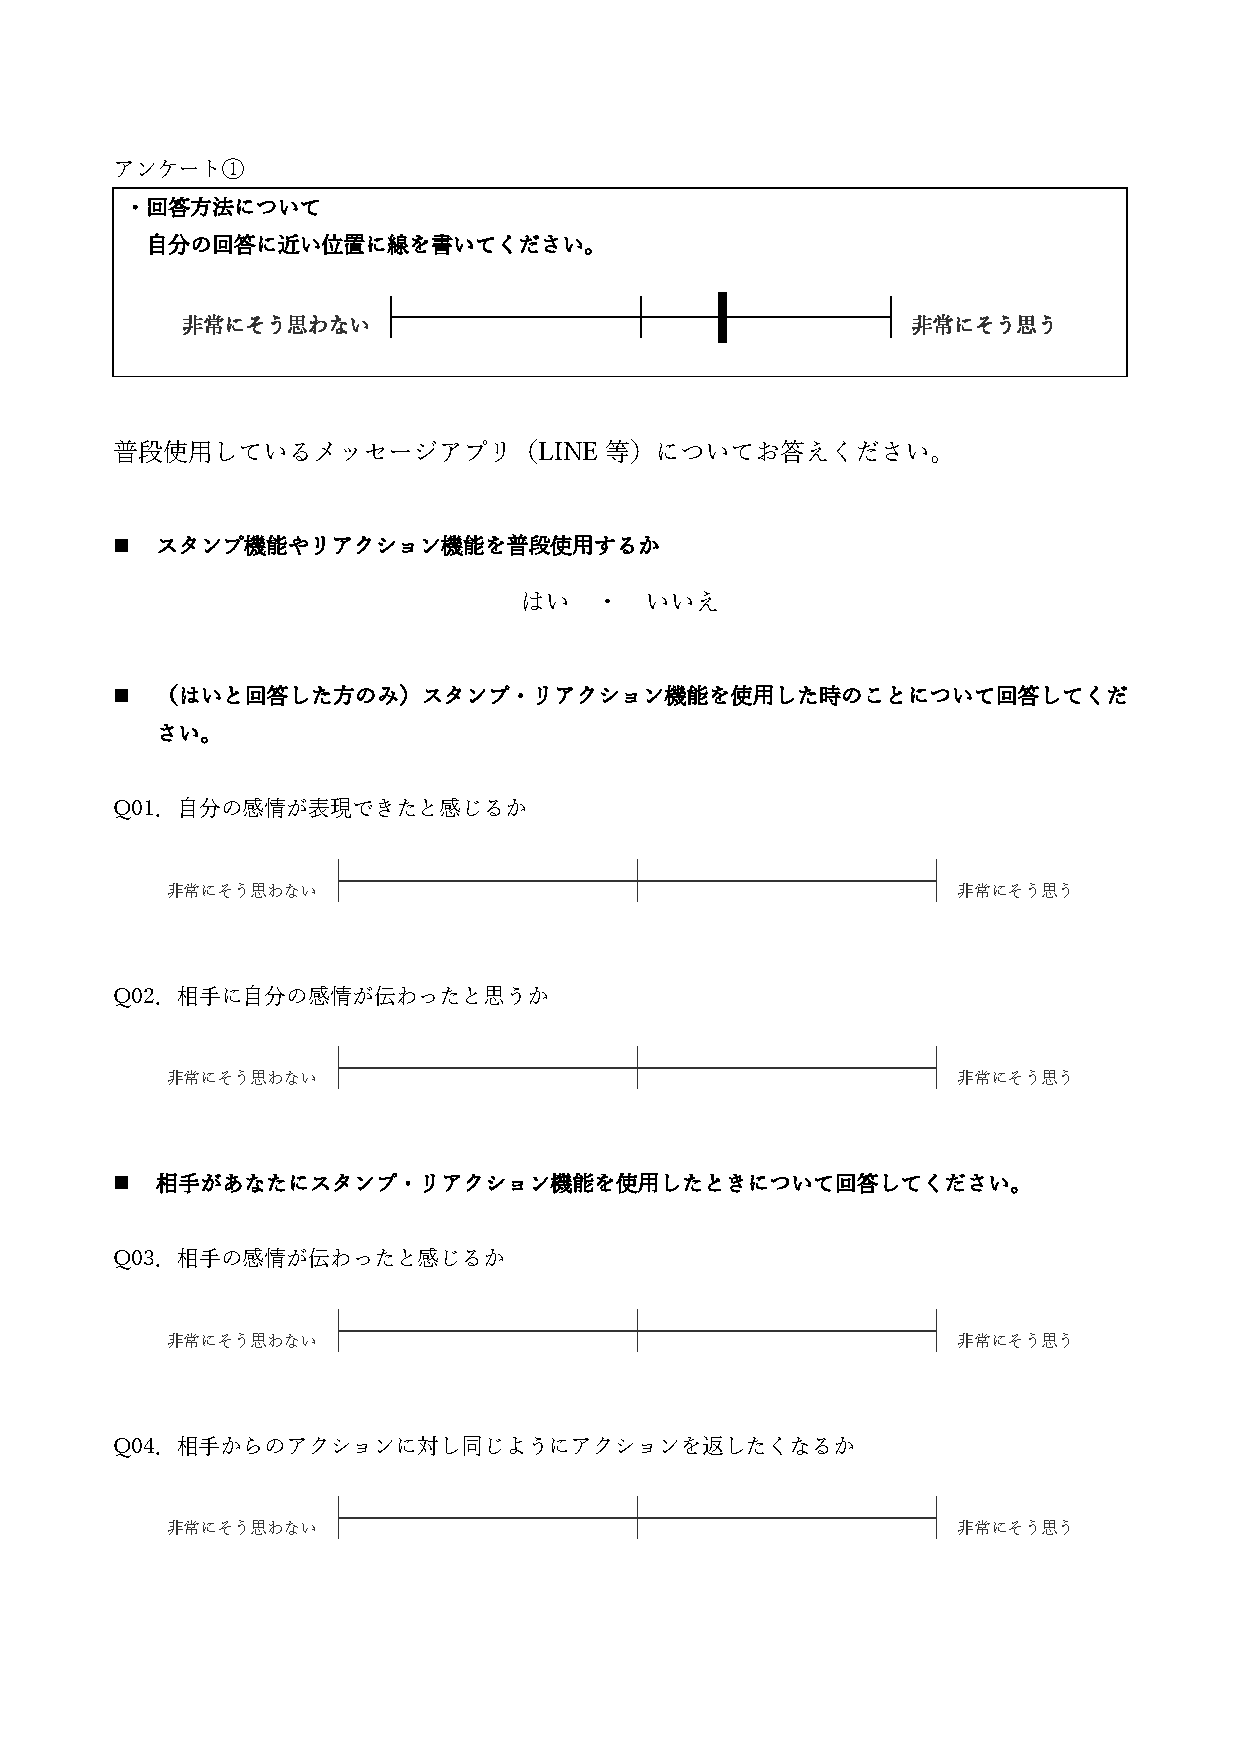
\includepdf[pages=-, scale=0.9]{PDF/questionnaire_1_ja.pdf}

\section{アンケート②}
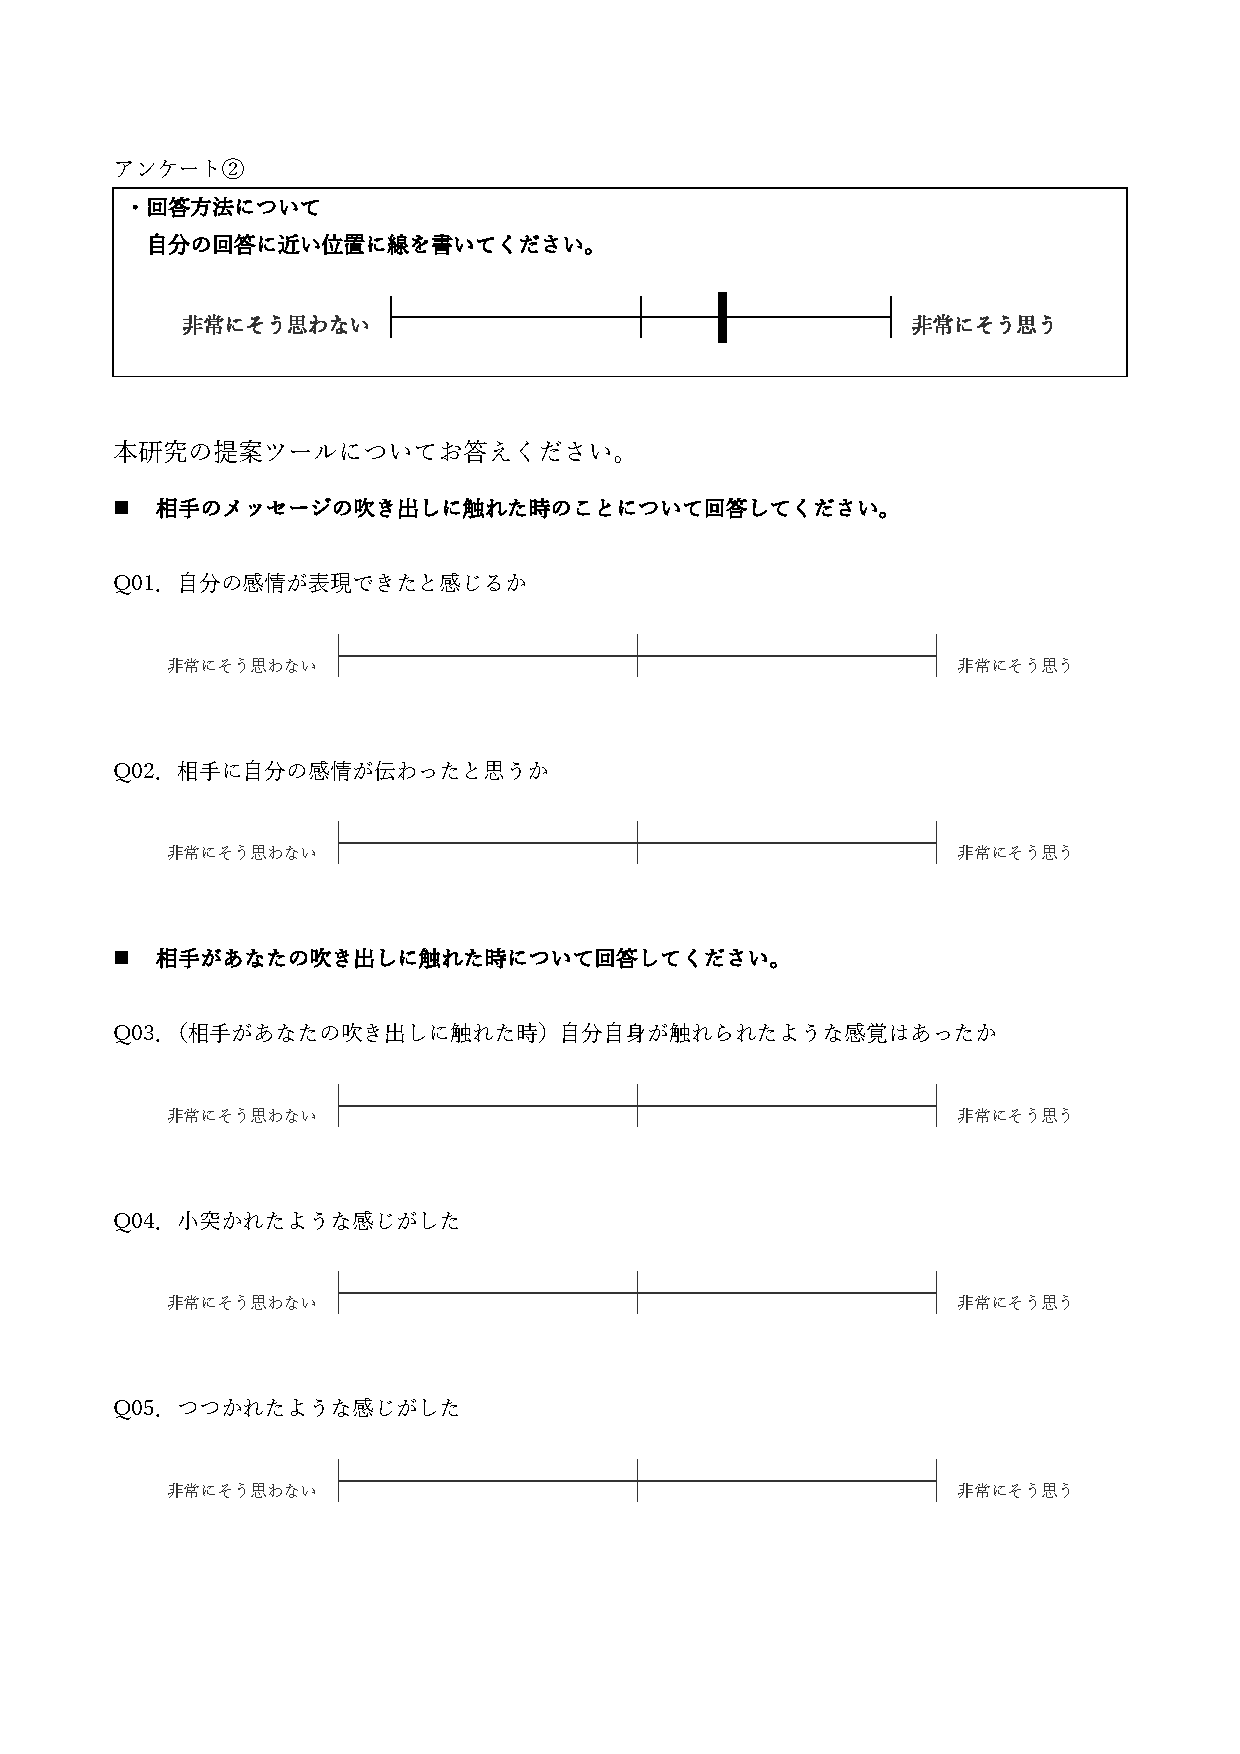
\includepdf[pages=-, scale=0.9]{PDF/questionnaire_2_ja.pdf}

\section{同意書}
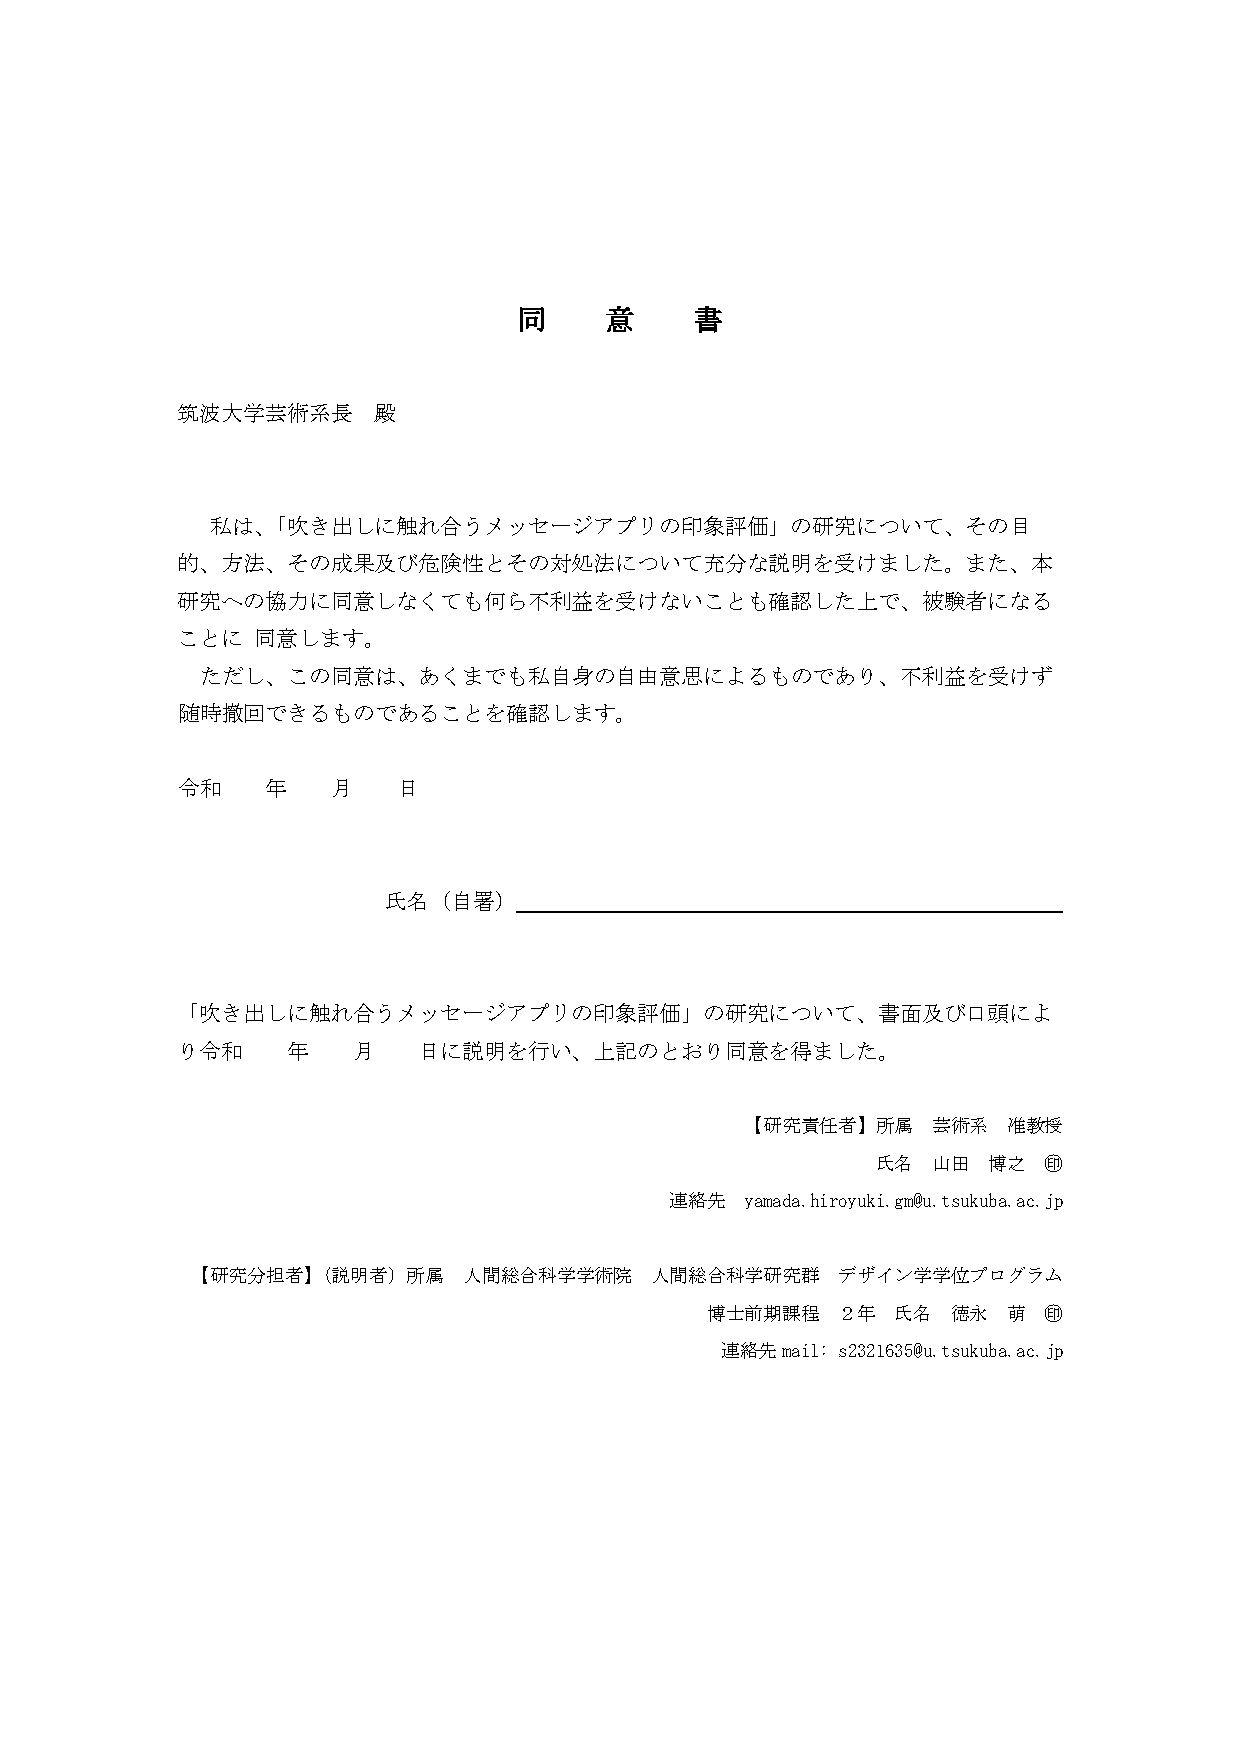
\includepdf[pages=-, scale=0.9]{PDF/agreement.pdf}

\section{同意撤回書}
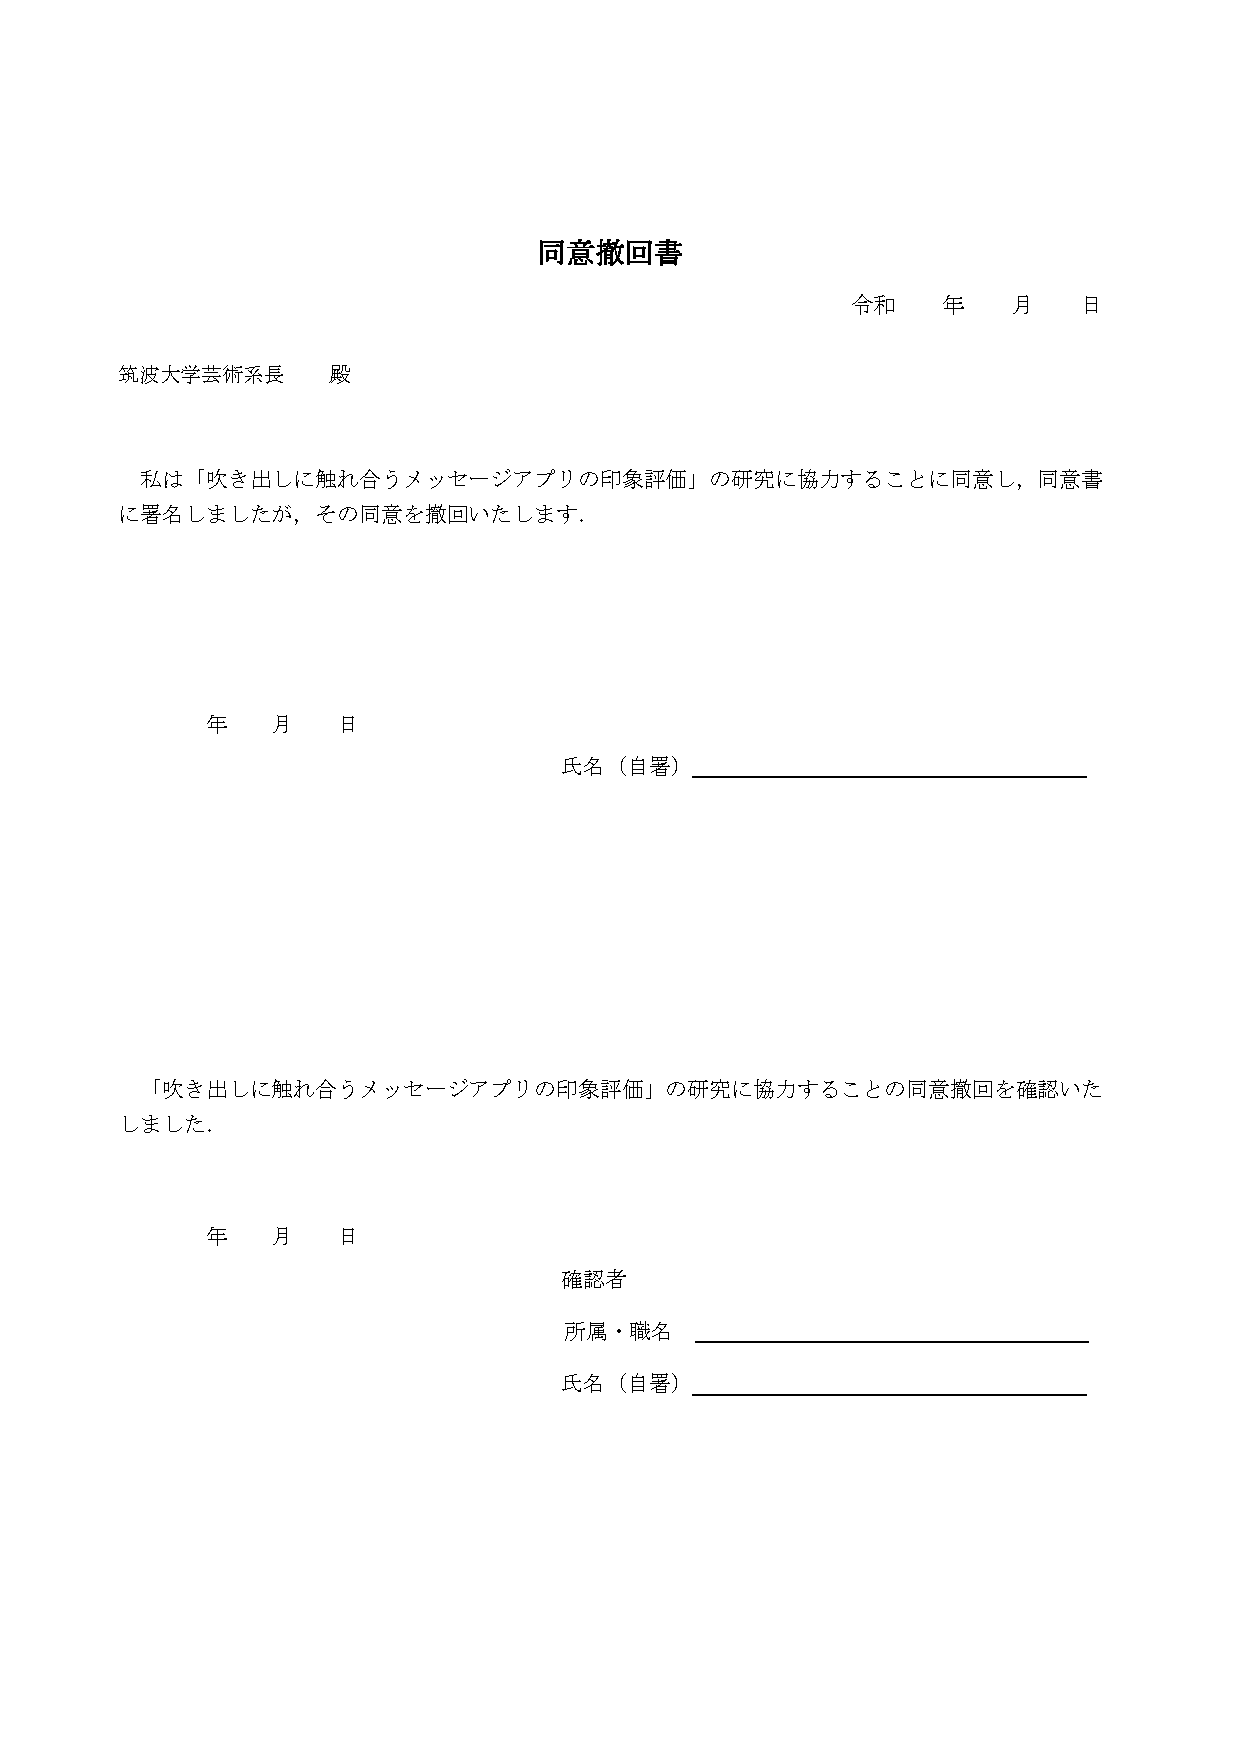
\includepdf[pages=-, scale=0.9]{PDF/withdrawal.pdf}

%------ここまで付録

\end{document}

%  卒業論文や修士論文を書くにあたって注意すべき点を挙げます。
%   \begin{itemize}
%       \item 参考文献の挙げる順序には,一貫性を持たせましょう。
%             よくある例としては以下のようなものがあります。
%       \begin{itemize}
%           \item 論文中での出現順(こちらのTeXサンプルは出現順になっています。指導教員の指示に従ってください)
%           \item 参考文献の筆者の名前順
%           \item 参考文献の出版年月順
%       \end{itemize}
%       \item 参考文献で挙げたものは,本文中で言及しなければいけません。
%       \item 参考文献番号はこんな感じでつけます
%   \end{itemize}

%------!!こちらの画像はTikZで作成してます。
% \vspace{5mm}
% \begin{figure}[htbp]
%     \begin{center}
%         \begin{tikzpicture}
%             \colorlet{myEgg}{gray!70!gray!50}
%             \draw[looseness=0.9,ball color=white!70!gray!50,draw=none,clip] (-2,0) arc (180:360:2) to[out=90,in=0] (0,3) to[out=180,in=90] (-2,0) -- cycle;
%             \foreach \x in {1,...,100}
%                 {   \pgfmathsetmacro{\rDot}{random()/50}
%                     \pgfmathsetmacro{\xCoo}{rand*2}
%                     \pgfmathsetmacro{\yCoo}{rand*2.5+0.5}
%                     \pgfmathsetmacro{\dColor}{100-60*sqrt(pow(\xCoo+0.5,2)+pow(\yCoo-1.4,2))/2.6}
%                     \fill[myEgg!\dColor!black] (\xCoo,\yCoo) circle (\rDot);
%                 }
%         \end{tikzpicture}
%         \caption{デザインした象の卵の形状}
%         \label{figure:elephants_egg}
%     \end{center}
% \end{figure}
%------!!

% 数式(\ref{eq:egg_equation})は、山本\cite{Yamamoto}が検討した卵形曲線の方程式のうちの一つである。

% \begin{eqnarray}
%     \label{eq:egg_equation}
%     (x^2 + y^2)^2 = ax^3 + (a - b)xy^2 \ \ \ \ \ (ただし、\ a \ge b \ge 0)
% \end{eqnarray}

% 論文に掲載した図表は必ず本文で説明すること。
% 一般的に図のキャプション(タイトル)は下に、表のキャプションは上につけます。
% 図表については、TeXのコード内で必ず\verb#\label{    }#を編集し、
% 図表番号も数字を記入せずに\verb#\ref{    }#を用いること。

% 図\ref{figure:Phoca_groenlandica}にタテゴトアザラシの赤ちゃんの写真を示す。
% この通り、愛らしい。
% 表\ref{table:SpeedOfLightTate}と


% ----- 図:タテゴトアザラシの赤ちゃん ------
% \begin{figure}[htbp]
%     \begin{center}
%         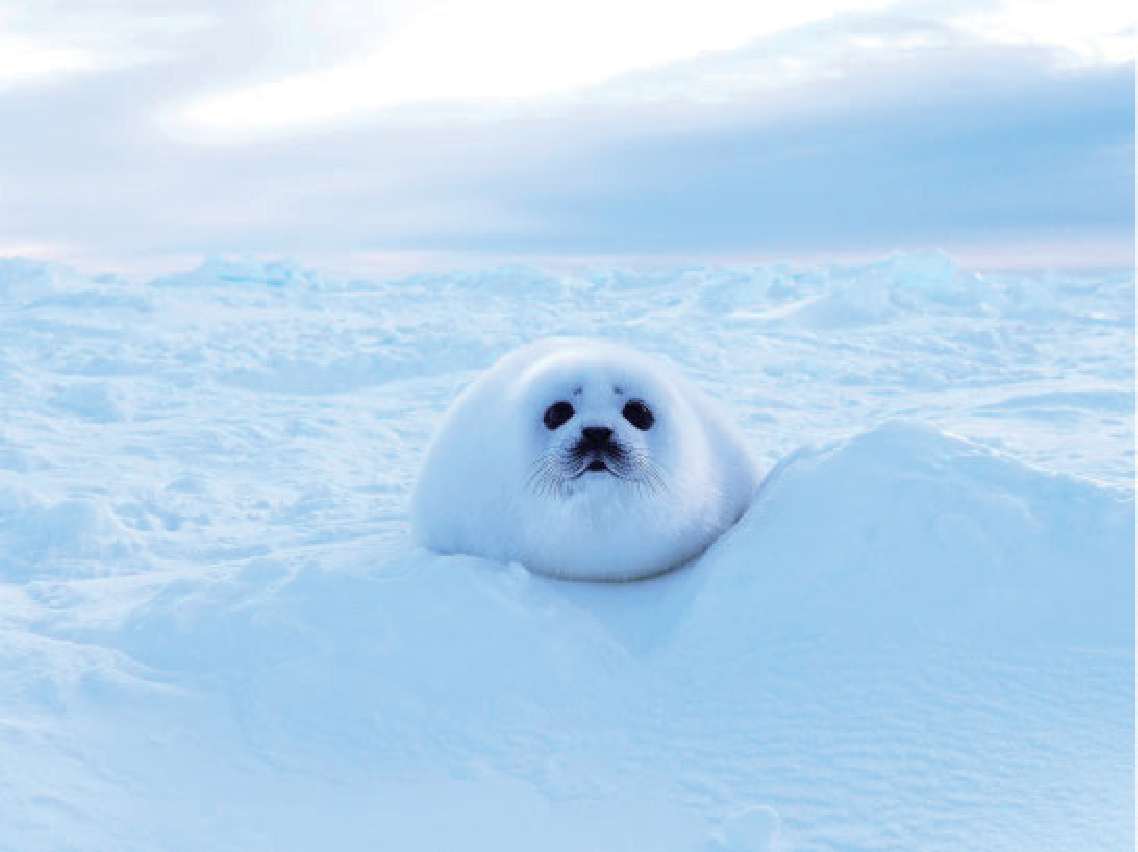
\includegraphics[width=100mm]{hoca_groenlandica.pdf}
%         \caption{タテゴトアザラシの赤ちゃん}
%         \label{figure:Phoca_groenlandica}
%     \end{center}
% \end{figure}
% -----ここまで図:タテゴトアザラシの赤ちゃん ------  

% -----表:光速度の測定の歴史 ------
% \begin{landscape}%表を90度回転させたい時にこれで囲む
% \begin{table}[!ph]
%     \caption{光速度の測定の歴史(横)}
%     \label{table:SpeedOfLightYoko}
%     \vspace{5mm}
%     \centering
%         \begin{tabular}{llll}
%         \bhline
%         病院名 & 取り組み & コンセプト & 課題 \\
%         \hline
%         1638 & Galileo & 二人が離れてランプの & (音速10倍以上) \\
%          &  & 光を見る &  \\           
%         1675 & Roemer & 木星の衛星の観測から & 2 \\
%         1728 & Bradley & 星の収差から & 3.01 \\
%         1849 & Fizeau & 高速に回転する歯車を通過する光を見る & 3.133 \\
%         1862 & Foucault & 高速に回転する鏡の光の角度変化 & 2.99796 \\
%         2022 & Aozora & 象の卵の疑似孵化実験から & 2.99792458 \\
%         \hline
%          \end{tabular}
% \end{table}
% \end{landscape}
% -----ここまで表:光速度の測定の歴史 ------ 
